\listfiles
\documentclass[link]{IWCOMP}
\usepackage{graphicx}
\usepackage{amsmath, amsthm, amssymb}
\usepackage{amsfonts}
\usepackage{tabularx}
\usepackage{multirow}
\usepackage{booktabs}
\usepackage[printonlyused]{acronym}
\usepackage{paralist}
\usepackage{enumitem}
\usepackage[ruled]{algorithm2e}
%\usepackage{algorithmic}

\setlist{nolistsep}

\newacro{PGCE}{Postgraduate Certificate of Education}

\newcommand{\tickYes}{\checkmark}
\newcommand{\crossNo}{$\times$}

\renewcommand{\newblock}{}

\copyrightyear{2021}

\DOI{xxxxxx}

% Document starts
\begin{document}

% Title portion
\title{Orchestrating Classroom Technology with Upper-Body Gestures}

\author{James McNaughton$^{1}$, Tom Crick$^{2}$ and Liz Burd$^{3}$}

\affiliation{$^{1}$Durham University, South Road, Durham DH1 3LE, UK \\
$^{2}$Swansea University, Computational Foundry, Bay Campus, Swansea SA1 8EN, UK \\
$^{3}$The University of Newcastle, University Drive, Newcastle NSW 2308, Australia}

\shortauthors{McNaughton, J., Crick, T. and Burd, E. }

\begin{abstract}
   There is a growing need to give teachers the ability to orchestrate technology in the classroom in an unobtrusive manner.
   The suitability of upper-body gestures for controlling classroom interfaces is considered in this work.
   A set of gestures intended to be intuitive to teachers is derived through the analysis of focus group outputs.
   The implications of implementing these gestures into a usable system are observed through the use of pilot study.
   Building on these observations, a full study is then carried out to assess the usage of the derived gestures in the classroom.
   The results of the study indicate that upper-body gesture controls are quicker and more intuitive than traditional orchestration technologies.
   However, the sensing technology used results in a high error rate which highlights a need for further improvements.
\end{abstract}

\keywords{Kinect, gestures, education, multi-touch, classroom technology}

\category{management decision-support system; teamwork; communication}

\editorial{Name}

\maketitle

\section{Introduction}
\label{sec:intro}

The uses of technology in the classroom are
growing~\cite{Schrum2008,Lloyd2011,Robertson2012},
further stimulated by significant reforms of digital skills and computer science education in various nations, especially across the UK~\cite{brown-et-al:toce2014}.
With this growth, the need for teachers to be able to control the deployed technologies increases~\cite{Apple1990,Selwyn2010,Selwyn2011}.
Without the ability to influence or control classroom technology, teachers may be unable to manage learning interaction or intervene when students start to lose focus on their current task~\cite{Chen2005,Karabenick2011}.

Many current systems that allow teachers to control technology in the classroom require the use of a teacher-centric interface~\cite{Dagdag2011,Kuhn2005,Vila2013,Zhou2010}.
Whether static, where the interface remains stationary during its use, or mobile, where the interface can be carried to new locations during its use, these interfaces require the teacher to momentarily take their attention away from the students.
This division of attention caused by the distraction of an interface could have a detrimental effect on the quality of a teacher's interaction with their students.
The disruption in communication between the students and the teacher this causes can be undesirable in many circumstances.
Therefore, a method of controlling technology in the classroom without breaking this interaction would be beneficial.
One such possible method is to make use of physical gestures, where a user performs an action which is identified by a monitoring system, to issue commands to technology in the classroom.

The use of gestures, rather than a more standard interface, could allow teachers to issue commands in a more effective manner.
Time is saved by not requiring the teacher to travel to their control interface.
Even when there is no travel time, such as when mobile interfaces are used, gestures have the potential to be executed quicker than alternative input and control methods~\cite{Dulberg1999,Moyle2001}.
Quicker execution of the commands should afford the teacher more time to observe and aid students.
In addition, physical gestures should be less intrusive on the interaction between students and the teacher. 
Many interfaces, specifically touch-screen mobile devices such as tablets, do not facilitate eyes-free interaction~\cite{Brewster2003}.
This means that teachers using a static or mobile interface which utilises a visual output are required to dedicate a portion of their attention to its use.
This division of attention can interrupt interaction between teachers and students.
The use of physical gestures should allow teachers to continue interacting with students while issuing commands to a classroom technology's control system.

Teachers in technology enhanced classrooms also acquire additional administration responsibilities~\cite{Kuhn2005} such as managing the consequence of faults with the devices used.
A physical gesture interface may reduce the overheads of such additional responsibilities by allowing teachers to quickly execute administrative tasks from any location in the classroom.
The potential benefits of physical gestures make its implementation into a classroom software framework desirable.

This paper investigates the implementation of physical gestures for use by teachers by utilising SynergyNet~\cite{HatchA.HigginsSMercier2009}, a multi-touch software platform intended for use in the classroom.
The platform is built to support applications intended for use by students through multi-touch interfaces.
SynergyNet contains a number of advanced networking features which support the sharing of materials~\cite{mcnaughton-et-al:jce2017} and the ability to issue commands to student devices through a network.

This paper documents the steps taken to augment the SynergyNet platform to use upper-body gestures, a subset of open-air gestures, to allow teachers to control classroom interfaces.
The paper also details the further steps taken to improve the experience of using the gestures in light of feedback.
These details of these steps, the reasoning behind them and their impact discussed in this paper have the potentional to benefit the future development of any systems with similar technologies, control sequences or gesture sets.

The remainder of this paper is as follows. 
Section~\ref{sec:background} discusses gesture detection technologies and approaches to gathering useful sets of gestures.
The issues in applying a gesture control to classroom orchestration is considered in Section~\ref{sec:issues}.
The creation of a solution which resolves these issues is then detailed in Section~\ref{sec:solutionDesign}.
A pilot study is presented in Section~\ref{sec:pilotStudy} which investigates the practical issues of implementing the proposed solution.
A study which then investigates the use of the devised solution is discussed in Section~\ref{sec:study}.
Overall conclusions and potential future developments based on the findings from the study are presented in Section~\ref{sec:conclusions}.

\section{Background} 
\label{sec:background}

% // TODO Needs more recent content.

To allow a system to identify physical gestures a method of tracking the movements of users is required.
Light-coding is a technique which can achieve this through detecting deformations in a projected pattern of light (usually infra-red) and using them to work out depth information.
There are several devices which support this technique such as the Canesta~\cite{Yang2007}, 3DV~\cite{Wilson2007a}, the Primesense sensor~\cite{Wilson2010} and the first generation of Microsoft Kinect.
These devices are not be confused with Time-of-flight cameras which use the time it takes for light shone by a device to be returned to build a depth-image ~\cite{Lange2001} such as the second generation of the Microsoft Kinect.

The firmware of devices which utilise light-coding offer several features relating to the tracking of a user.
These devices can outline any persons in front of the device and differentiate between them using their distances from the camera.
The device can then identify and give positional information on specific parts of a person's body, such as their limbs and joints if a calibration technique is executed.
This is usually a pose assumed by a person which allows the device to view a specific human outline from which it can identify joints and limbs~\cite{Xia2011}.
Using the difference between frames from the depth camera, the device's firmware can track the movement of people in its field of view.

The information a light-coding device can give concerning the positions of a person and their limbs offers a wealth of possibilities regarding computer interaction.
Specifically, the ability to obtain the positional information of people may be of use for co-located interfaces where interaction may require knowledge of the position of the user.
The ability to track and differentiate between users comes in useful for interaction technologies which allow users to share interfaces.
Dietz and Leigh~\cite{Dietz2001} note how the ability to track a user can be important.
Their research also identifies how existing techniques for tracking user positions which entail encumbering the user with extra devices are undesirable.
Light-coding devices offer the opportunity to track people without the need for users to wear additional devices.

Devices which can track the movement of user allow for movement about an environment without being constrained to an interface.
This is beneficial for teachers in classroom environment for whom mobility is vital.
There are alternatives to physical gesture sensing technologies which also afford this type of freedom from the interface.
Voice control is one such alternative where the teacher could issue commands to a technological framework in the classroom through a series of spoken instructions.
Using physical gestures alongside the voice commands could be beneficial as shown in the work of Bolt~\citeyearpar{Bolt1980}.
Allowing the user to gesture at where they want a specific command to influence reduces the need for additional spoken instructions.
However, the ambient noise in a typical classroom is likely to be too loud for voice recognition technologies~\cite{Cavalier1996,Goette1998,OHare1999}.
In addition to this caveat, the issuing of voice commands also will require teachers to interrupt their conversations with their students.

The use of physical gestures monitored via a light-coding device appears to be the most suitable approach to creating a system which allows teachers to control classroom technologies without the requirement for a distracting interface.

\section{Issues with Gesture-Driven Classroom Technology Orchestration} 
\label{sec:issues}

Light-coding devices could allow teachers to control technology in the classroom without the need for a physical interface.
Since physical gestures would permit eyes-free interaction~\cite{Brewster2003} with a control system, teachers could interact with students without losing control of the technology.
Due to a light-coding device's ability to track people in an environment, once a teacher is identified their movement around the classroom can be followed.
As a result of this, teachers could potentially issue commands through gestures from anywhere in the classroom.

Light-coding devices have high availability and relatively low cost in comparison to alternative depth sensing devices such as those used in Oblong's Mezzanine~\cite{kramer2011}.
Despite these potential benefits of light-coding device, there are several limitations that must be considered.
One limitation is their accuracy.
Light-coding devices are capable of tracking users and the position of their limbs.
However, for a light-coding device to track anything more precise, such as fingers, additional constraints on their abilities will need to be imposed \cite{Clark2011}.
These additional limitations potentially include a reduction in range, a reduced limit on the number of tracked users and the use of encumbering devices.
All these limitations are undesirable for the use of the device in the classroom.
Therefore, in the work discussed here, light-coding device will be assumed not be augmented to track anything more precise than user limbs.
This means that any gestures to be used by teachers for issuing control commands should consist of limb positioning and movement.

The inability of an un-augmented light-coding device to track anything more precise than user limbs discounts the adoption of gestures which use fingers for use in the classroom.
There are several reasons for gestures involving the use of the lower body limbs and joints, such as the legs, to be discounted also.
One such reason is their requirement for the visibility of the lower body.
In a classroom full of furniture and seated students, the teacher's lower body will potentially be obscured most of the time from the view of the light-coding device.
Due to these reasons, only gestures which utilise the positioning and movement of the upper-body should be considered when developing a classroom control system.
This means that gestures should only make use of upper-body joints and limbs which a light-coding device can track: the torso, wrists, hands, elbows, shoulders, neck and head.

\subsection{Considerations for Light-Coding in the Classroom}  
\label{subsec:considerations}

The use of physical gestures in the classroom requires that several considerations are taken into account in the design of any system which supports them.

\subsubsection{Avoiding False Positives}  
\label{subsubsec:falsePositives}

A potential issue concerning light-coding devices are that, by default, they are active at all times.
This means that teachers will need to be mindful of their actions.
Expressive body language or movement around the classroom could be interpreted by a light-coding device as a gesture.
This may trigger unwanted responses from any system utilising the device.
Therefore, a method of dismissing a light-coding device's attention and recapturing it later would be beneficial 
One potential solution to these false positives is to have designated areas from which gestures should be made.
This would allow teachers to move outside these areas without the possibility of accidentally issuing a command.
However, this solution does restrict the locations where the commands can be issues from, diminishing the ability of teachers to issue commands from anywhere.

A gesture based method of toggling a light-coding device's attention is another potential solution to the issue of a teacher unintentionally issuing commands through their movement in the classroom.
The light-coding device will not be able to issue any commands to a classroom technology unless its attention has been obtained by the teacher.
This results in the light-coding device used having two states: attentive and inattentive.
A gesture could be setup to be identified by the light-coding device in both states.
This gesture can be used to toggle state.
This diminishes the range of possible false gestures to one.
The solution reduces the chances of a teacher unintentionally issuing commands and allows for control over the light-coding device anywhere in the environment.
If this solution is adopted it is important to identify the gesture for gaining and dismissing the light-coding device's attention.

A potential drawback with the attention-toggling approach of managing these false positives is that if a teacher intentionally performs a gesture without getting the device's attention they will be ignored.
A false negative is preferable to a false positive because an unintended gesture may have irrecoverable consequences.
A false positive will have no consequence other than requiring the teacher to repeat their gesture again with the attention of the light-coding device.
Despite not being as problematic as the potential consequences of a false positive, the time-wasting result of a false negative is a potential issue.
A method of ensuring that a teacher knows whether they have the light-coding device's attention would be beneficial in stopping false negatives if the attention-toggling approach is taken.
Audible or visual feedback would aid the teacher in knowing whether their movement can or cannot be interpreted by the system as a gesture.

\subsubsection{Interface Selection}  
\label{subsubsec:interfaceSelection}

It is important to note that sometimes a teacher may wish to issue a command to specific selection of devices in the classroom rather than all.
This means that the teacher should be able to perform a gesture in such a way that the system is informed that the related action is intended to only affect specific devices.
A light-coding device's ability to track users can allow for the system to be informed of the location of a teacher in relation to the interfaces in the classroom.
Therefore, the teacher's proximity to interfaces could be used by a system to identify which devices a command should affect if informed of their locations.
However, the drawback to this approach is that if the teacher wishes to influence multiple interfaces they will be required to repeat the gesture in close proximity to each of the target interface which could take up an undesirable amount of time.
An alternative could be to use a specific gesture which can communicate a preferred device, or devices, to the system.
If implementing this into the design of a gesture set it is important to ensure this gesture is quick to perform and intuitive as it is likely to be repeated often by the teacher.


\section{Designing a Solution for Gesture-Driven Classroom Orchestration} 
\label{sec:solutionDesign}

With all the requirements for using gestures in the classroom and the limitations of the most suitable technologies outlined in Section~\ref{sec:issues} an important question becomes apparent:
\emph{Are gestures a viable method for controlling technology in the classroom?}

To answer this question a system for using gestures in the classroom first needs to be designed and implemented.
As part of the design a suitable set of gestures needs to be generated.
To inform the creation of the gesture set a focus group is utilised to find a set of relevant and un-intuitive gestures.
With a suitable set of gestures, a system which utilises them in the classroom can then be produced.
A study which utilises this system can then be used to answer the question of whether gestures are a suitable control technology for the classroom.

The requirements of the set of gestures to be used by teachers in the classroom are determined by both the shortcomings of the sensing technology, as discussed in Section~\ref{sec:issues}, and the abilities of the intended users.
Specifically, the set of gestures for controlling classroom technologies are those which are able to be detected by a light-coding device and are suited to be performed by teachers.
With the potential set of suitable gestures already reduced to the upper-body by the requirements of using the sensing technology in a classroom environment, there is now the task of identifying which gestures to use and with which controls.

\subsection{Gathering User Generated Gestures} 
\label{subsec:gatheringGestures}

It is important that the gestures selected for use in the study are intuitive~\cite{Cohen2002,Wachs2011} to allow teachers to easily remember gestures and perform them with minimal forethought.
Its also important that the number of gestures is kept small to avoid difficulties with requiring users to remember too much so that frustration with using the system can be minimised~\cite{Mendoza2005}.
The typical adult can remember seven items in a list, give or take two, in their short term memory~\cite{mil56}.
Relying on committing a greater number of commands to long term memory is undesirable since it counters the benefit that intuitive gestures offer of being quick to learn and use.

A framework for assessing potential gesture sets for the study must be decided upon.
An exhaustive literature survey utilising a structured protocol~\cite{kitchenham04} revealed that no framework currently exists for the evaluation of gestures meeting the requirements of classroom orchestration with upper-body gestures as outlined in Section~\ref{sec:issues}.
Therefore, an evaluation framework used for a similar set of gestures was required to be identified and adapted.

Nielsen et al.~\citeyearpar{Nielsen2004}'s work on procuring suitable sets of gestures for ergonomic interfaces entails the assessment of gestures using a framework of characteristics.
This framework is derived from a combination of usability principles and heuristics derived from ergonomic theory.
The characteristics the framework uses for assessment are a gesture's; (i) ease to perform and recall, (ii) intuitiveness, (iii) logical metaphoric and iconic links towards functionality and (iv) ergonomic nature.
Waches et al.~\citeyearpar{Wachs2011} outline a series of requirements which systems using hand-gestures should adhere to, a number of which echo the characteristics used in Nielsen et al.~\citeyearpar{Nielsen2004}'s work.
In addition to these are additional requirements which relate to the sensing technology used which relate to the technologies to be used in the study.

Because of their relevance it was decided that the requirements outlined by Waches et al.~\citeyearpar{Wachs2011} would be adopted for use to assess gestures in the study.
The more technical requirements and how a typical light-coding device adheres to them are as follows:

\begin{itemize}
\item  \textit{\textbf{Cost:}} As detailed in Section~\ref{sec:issues}, light-coding devices are relatively low cost.
\item \textit{\textbf{Responsiveness:}} The Kinect, a light-coding device, has a frame rate of 30Hz~\cite{Livingston2012} which is enough to be considered adequately responsive for tracking the movement of users.
\item \textit{\textbf{Adaptability:}} A typical light-coding device has the ability to be used by various supporting software frameworks which each allow accessing of the device's collected data and functions~\cite{Goth2011}.
This allows light-coding devices to be easily adapted for changes in use.
The scalability of a single light-coding device to track the joints and limbs of multiple persons is a demonstration of its ability to adapt to different numbers of users.
\item \textit{\textbf{Accuracy:}} The Kinect, a light-coding device, is noted to track user's limb and joints to 20mm when in range~\cite{Marquardt2011}.
\item \textit{\textbf{Un-encumbering nature:}} When a user is required to wear a device for some purpose, the affiliated system is considered to be encumbering.
This can be undesirable as it detracts from a system's ubiquity and may impede use. 
Since a light-coding device can track users through a single static device which does not need to be worn it is considered to be un-encumbering.\\ 
\end{itemize}

One of Waches et al.'s~\citeyearpar{Wachs2011} requirements refers to the gesture set itself.
A criterion based on this requirement can be stated as follows:

\begin{itemize}
\item \textit{\textbf{Lexicon Size:}} The size of the gesture set must not be too large.
This criterion can be adhered to by taking into account the limitations of short term memory.\\ 
\end{itemize}

The remainder of the requirements outlined by Waches et al.~\citeyearpar{Wachs2011} refer to requisites of the hand gestures themselves.
A summary of these criteria for upper-body gestures based on these requirements can be outlined as follows:

\begin{itemize}
\item \textit{\textbf{Intuitiveness:}} A gesture which a user performs naturally in relation to a specific command action is beneficial.
\item \textit{\textbf{Comfort:}} If a gesture is uncomfortable to perform a user is unlikely to perform it frequently, thus diminishing the benefit of the system.
\item \textit{\textbf{Low mental load:}} For a gesture to conform to this criterion a user should be able to perform it with little forethought.
\item \textit{\textbf{Interaction space:}} Gestures which require large amounts of space to be performed limit the locations it can be performed.
Therefore, to fulfil this requirement, gestures should minimise used space.
\item \textit{\textbf{Ubiquity:}} A gesture which does not appear to be in keeping with a user's typical actions in the current environment would not fulfil this criterion. \\ 
\end{itemize}

Using these criteria, any suggested gesture sets and their suitability can be assessed to be viable or not.

\subsection{Focus Group} 
\label{subsec:focusGroupDesign}

To discover gestures which conform to the criteria outlined in Section~\ref{subsec:gatheringGestures} a user-centred design process was adopted.
As part of this process a user study in the form of a focus group was organised.
Through the focus group a user-generated set of viable upper-body gestures for use with a light-coding device was discovered.
The focus groups acted as a form of guessability study~\cite{Ruiz2011,Wobbrock2009} which would generate gestures which are natural to the user~\cite{Grandhi2011}.
User-generated gestures for surface computing are noted to be intuitive, comfortable, memorable and ubiquitous~\cite{Bjorneseth2012}.
These potential benefits of user-generated gestures adhere to the criteria relating to the definition of effective upper-body gestures.

The primary objective of this study was to find the quickest, most intuitive and least intrusive upper-body gestures which can be performed in the classroom to execute the most important control commands.

Three focus group sessions took place.
All participants were required to have had some experience of teaching in a classroom environment.
Participants were asked to position themselves in the room used in the study facing away from each other and towards the cameras recording the session to reduce the influence that they would have on each other.
In each session a number of the participants were asked to stand and the rest were seated.
A list of commands that teachers using a classroom control system may need to issue was compiled.
The commands used were those for: 
\begin{itemize}
\item Freezing/Unfreezing student interfaces.
\item Sending contents of student interfaces to a shared interface.
\item Sending contents of a board interface to student interfaces.
\item Showing snapshots on the board interface of the student interfaces.
\item Clearing the student interfaces.\\
\end{itemize}

These commands were decided upon based on observations on which were the most frequently issued during previous studies~\cite{Hatch2011}.
It was decided to adhere the lower bound of short term memory, discussed in Section~\ref{subsec:gatheringGestures}, of five.
This relatively small gesture set conforms to the Wachs et al.'s~\citeyearpar{Wachs2011} requirement for a small lexicon size.

For each command participants were asked to perform the first gesture that they thought of which related to it meaning  that the gestures performed were likely to be natural to the participant.This is beneficial for finding gestures which conform to the criteria outlined in Section~\ref{subsec:gatheringGestures}.
Spontaneous and frequently repeated gestures are assumed to be natural to the user and therefore are \textit{\textbf{intuitive}}~\cite{Grandhi2011}.
The intuitive nature of the gestures also implies that they are \textit{\textbf{comfortable}} for participants to perform.
Since participants were asked to put little thought into their motions, the gestures can also be said to have a \textit{\textbf{low mental load}}.
Participants were placed closely side-by-side helping ensure that the gestures used would utilise a restrained \textit{\textbf{interaction space}}.
Participants were also asked to be mindful of the fact that these gestures would be performed in a classroom environment to ensure that the gestures suggested by participants would be in some part \textit{\textbf{ubiquitous}} to the classroom environment.

Participants in the study were asked to perform two gestures for each command.
The first gesture related to a command issued to all interfaces whereas the second related to a command intended for a specific selection of interfaces.
Participants were made aware that gestures should only use the upper-body but not fingers and that a gesture can either be a pose or movement.
Participants were also informed that they could not assume their promiximity to a device could not be used for selecting a specific interface.

\subsubsection{Focus Group Data Analysis}
\label{subsubsec:focusGroupDataAnalysis}

Using video recordings of the focus group sessions all participants' movements for each command could be studied and summarised as a sequence of poses and movements.
This allowed the participants' actions to be formalised as gestures.
These gestures could then be compared, allowing similar actions to be identified as being separate instances of the same gesture.
The gestures which were used most frequently for specific commands could then be identified.
The most frequently occurring gesture for a command is likely to be the most intuitive since they will match the intended users' mental model of how the system should be used~\cite{Nielsen2004,Ruiz2011,Wobbrock2009}.

Each unique gesture identified was first evaluated against the limitations of a typical light-coding device.
Any gestures which did not conform to these limitations, such as those which used finger motions, were discounted.
Following this, the criteria outlined in Section~\ref{subsec:gatheringGestures} were used to assess the gestures.
Any gesture which did not meet the criteria was also discounted.
The viable gestures observed for a command across all the sessions were then ranked by frequency to identify those to be considered most intuitive.

If more than one command had the same gesture with the highest frequency, the gesture would be assigned to the command with the highest usage observed in past studies~\cite{HatchA.HigginsSMercier2009}.
The less used commands would then be assigned their gesture with the next highest frequency.

It was decided that the attention toggling method of managing false positives, discussed in Section~\ref{subsubsec:falsePositives}, would be adopted due to its ability to reduce errors without placing constraints on where in an environment gestures can be performed.
Every effort was made to ensure participants' minds were kept clear of any assumptions about the system to aid the performance of intuitive gestures~\cite{Nielsen2004}.
As part of this effort it was decided that the participants should not be made aware of the toggle mechanic.
Since this gesture potentially needs to be performed prior to any other command gesture, it will be the most frequently used in the system.
Therefore, the most frequently occurring gesture throughout the entire study was chosen for this mechanic to ensure that is is intuitive and natural.

The data analysis also aimed to identify how the participants differentiated gestures intended for all interfaces from those intended for specific interfaces.

\subsection{Focus Group Results}
\label{subsec:focusGroupResults}

Of the sixty seven participants who took part in the study, fifteen were male and fifty two were female.
This was representative of the gender balance of \ac{PGCE} students at the institution.
The majority of these participants were aged between twenty and twenty five.
The video recordings from the study were analysed by the first author.
From the analysis of the videos, several patterns in the participants' gestures were observed.

\subsubsection{Toggling Attention}
\label{subsubsec:focusGroupResultsTogglingAttention}

The most common gesture was a simple horizontal wave of a single hand.
Seven percent of all gestures observed in the study comprised of the waving of a single hand.
This was used by participants frequently and may have been a gesture for actions where the participant could not think of an appropriate gesture. 
While some participants would not perform a gesture for commands that they could not think of a suitable gesture for, others would instead perform a generic gesture, referred to as a \textit{default gesture}.
This set of default gestures were not specific to any particular subset of commands but were frequently used by participants.
In addition to waving with one hand these default gestures included; holding one hand up and pointing with one hand.
These gestures accounted for twenty eight percent of the observed gestures in the study.

\subsubsection{Interface Selection}
\label{subsubsec:focusGroupResultsInterfaceSelection}

7\% of the study's participants showed no clear method of differentiating between commands that affect all interfaces or those which affect specific interfaces. 
These participants would either repeat the same gesture for both instances of the command or would have no single consistent differentiation approach for the commands. 

To differentiate between commands which affect all interfaces and those which affect specific interfaces, 93\% of the participants would always follow a consistent approach.

\begin{itemize}

\item \textbf{Use two completely different gestures.}\\
A minority, 23\% of participants, would always perform different gestures as a method of differentiating a command applied to either all or specific interfaces.
This differed from the majority who would use the same gesture for a command when applied to all or specific interfaces with a slight deviation between them.
A drawback with the approach of using different gestures is that it effectively doubles the number of gestures a teacher must remember since each command would have two gestures affiliated with it.
This would increase the number of gestures to ten which is unacceptable since it may to be large for many potential users' short-term memory.
Another drawback to this approach was that the gesture intended to affect specific interfaces would be required to utilise the light-coding device's user tracking ability to determine which interface the teacher is closest to.
This would require the teacher to repeat the gesture for all interfaces they wish to the command to be applied to making the issuing of commands take significantly longer.

\item \textbf{Use different sized versions of the same gesture.}\\
5\% of participants were noted to perform the same gesture for issuing a command but would differentiate between whether it would affect all or a specific subset of interfaces through the size of the gesture.
The size of the gesture is defined by the amount of space that it occupies.
For example, some gestures involved the user drawing a circle with their hands.
For what would be considered a small gesture for some participants, this circle would have a diameter under half a metre.
For these participants a large version of the gesture would entail the user drawing a circle with a diameter larger than half a metre.
For all participants using this approach, the small version of a gesture was applied to the command affecting only specific interfaces.
For this approach to be implemented, the small gesture would have to use the teacher's proximity to the interfaces to determine which to affect.

\item \textbf{Perform the gesture with either one or two hands.}\\
Another approach adopted by participants for differentiating between a command that affects all interfaces or specific interfaces was defined by the number of hands used. 
The 8\% of participants who followed this approach constantly throughout the study would all use a single hand to perform gestures intended to affect specific interfaces.
These participants would then perform the same gesture with both hands when applying the command to all interfaces.
This approach, like that which utilises the size of the gesture, requires teachers to repeat the one-handed version of a gesture in close proximity to all the interfaces they wish to affect.

\item \textbf{Perform the gesture and pointing at the interfaces it should affect.}\\
The majority of participants, 57\% in total, would perform a pointing gesture to signify a command affecting specific interfaces.
This pointing gesture would be where participants locked their arm in a straight line.
Some of the participants performing this gesture would also point with a finger but this would be ignored by a sensing technology as inaccurate as a light-coding device.
Participants who adopted the approach of pointing at the interfaces they wished to affect would perform the command gesture on its own when wishing to issue the command to all interfaces.
This was the most popular method of differentiating between whether a command should affect all or specific interfaces.
3\% of participants who adopted the pointing approach would always perform the gesture with one hand and point with the other throughout.
Alternatively, participants would perform the command and pointing gestures sequentially.
All of these participants would point first and then perform the gesture.

\end{itemize}

\subsubsection{Command Gestures}
\label{subsubsec:focusGroupResultsCommandGestures}

Noted in the analysis was that despite many of the gestures being one handed, participants did not use handedness to distinguish between single hand gestures for various commands.
Participants may have considered that a gesture which is required to be used with a specific hand may be problematic for those whose handedness differs from their own.
This implies that hand-dominance did not influence which gestures participants considered for the commands.

\begin{figure*}[p]
   \centering
   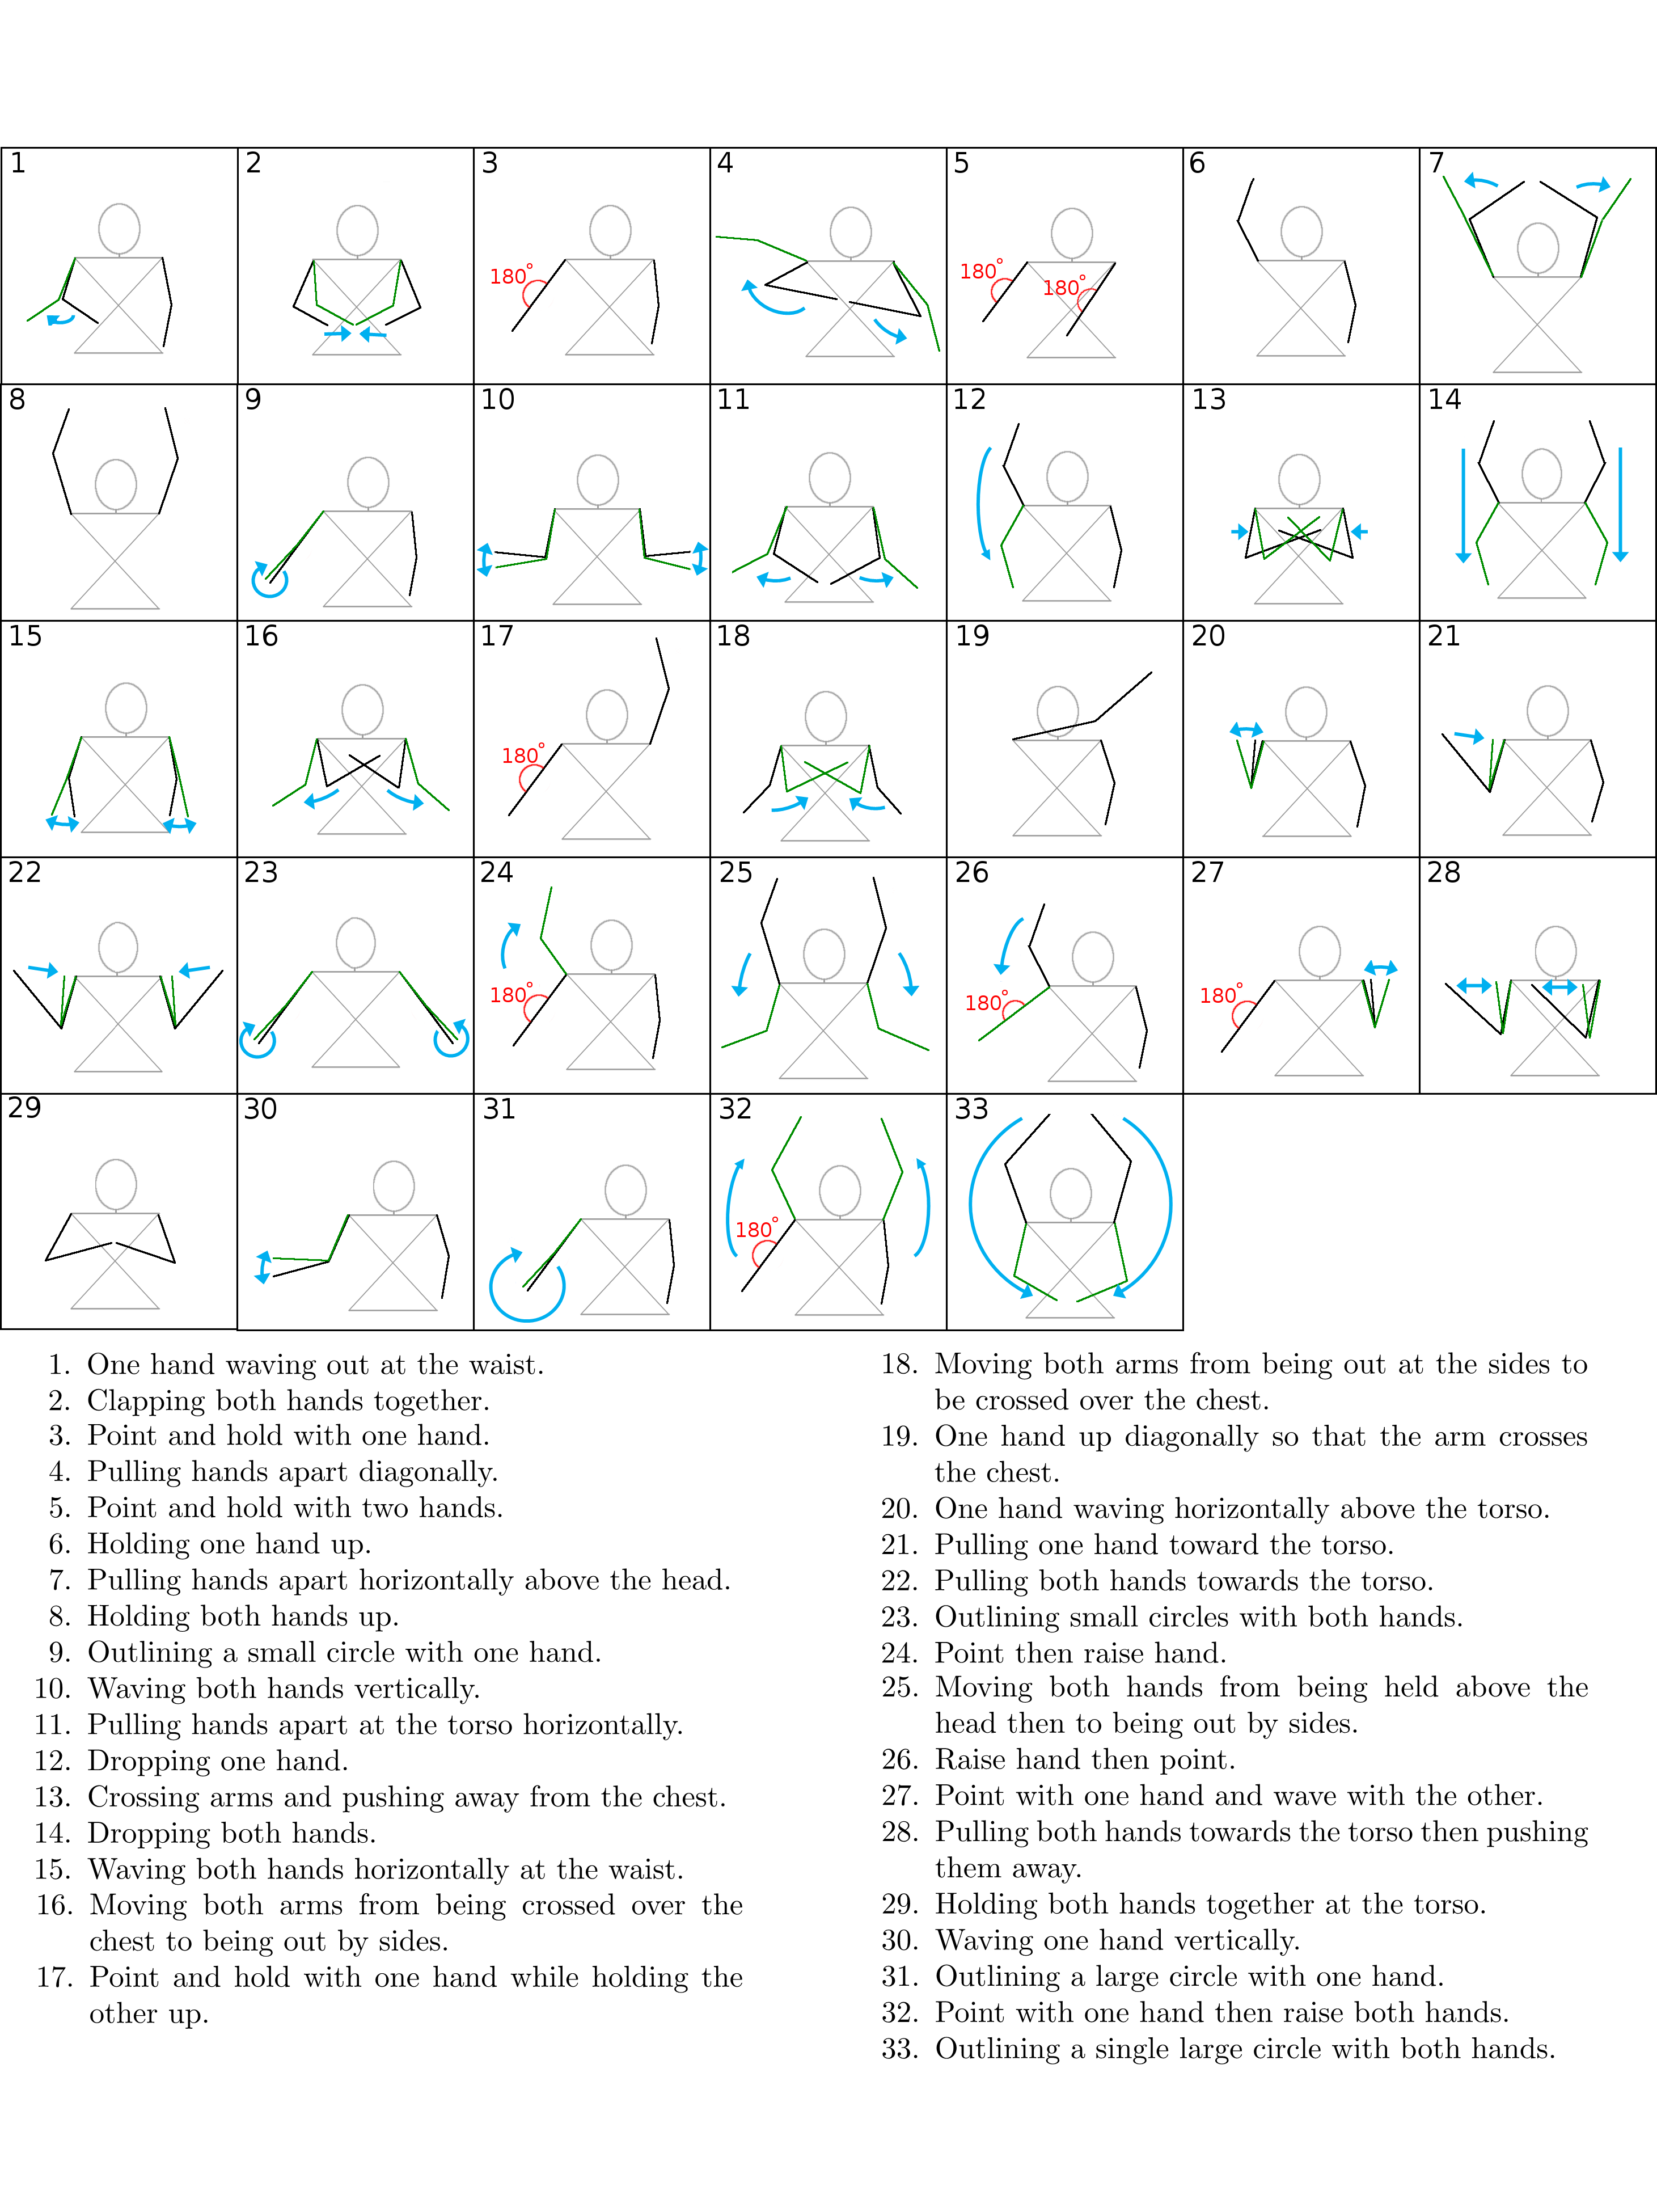
\includegraphics[width=1\textwidth]{figures/all_gestures.png}
   \caption{All unique gestures observed during the study.}
   \label{fig:allGestures}
\end{figure*}

Thirty three unique gestures which conform to the criteria outlined in Section~\ref{subsec:gatheringGestures} were observed during the study.
These gestures are shown and described in Figure~\ref{fig:allGestures}.  

After reviewing the videos and attaining the number of occurrences for each gesture per command over all the studies, the most frequently used gestures for each command could be identified.
Popularity refers to the gestures frequency of occurrences and was used as it often indicates intuitiveness~\cite{Grandhi2011}.
The results are as follows: \\

\begin{itemize}

\item \textbf{Freezing/Unfreezing the classroom interfaces.}\\
\textit{Gesture 8: Holding both hands up.}\\  
10.65\% of the gestures performed for this command exclusively entailed participants holding both hands up.
The popularity of this gesture for the freeze command is likely due to its similarity with the commonly used halt or stop hand signal.\\

\item \textbf{Sending contents of the classroom interfaces to the board.}\\
\textit{Gesture 6: Holding one hand up.}\\
1.12\% of the gestures performed for this command exclusively entailed participants holding a single hand up.
There were so many unique gestures performed for this command that even the more popular gestures had only a small share of the total.
Though holding a single hand up was popular amongst many of the participants for a variety of commands, it proved to be most popular for sending contents to the board.\\

\item \textbf{Sending contents of the board to the classroom interfaces.}\\
\textit{Gesture 21: Pulling one hand towards the torso.}\\
15.49\% of the gestures performed for this command exclusively entailed participants pulling a single hand towards their torso.
This gesture was likely popular because the motion gives the appearance of the teacher beckoning content from the board, effectively pulling it towards the classroom interfaces.\\

\item \textbf{Showing snapshots on the board of the classroom interfaces.}\\
\textit{Gesture 29: Holding both hands together at the torso.}\\
10.26\% of the gestures performed for this command exclusively entailed participants holding both their hands together near their torso.
Many participants made a gesture with their fingers for this command emulating taking a photo on a camera.
When asked to modify their behaviour so that they did not use their fingers (due to the limitations of light-coding devices discussed in Section~\ref{sec:issues}) participants often performed Gesture 21 instead.
This gesture is as close to emulating taking photos as possible without the use of fingers.\\

\item \textbf{Clearing the classroom interfaces.}\\
\textit{Gesture 11: Pulling hands apart at the torso horizontally.}\\
48\% of the gestures performed for this command exclusively entailed participants pulling both their hands apart near their torso.
This gesture was likely popular due to its similarity to the real life action of sweeping objects off a surface.
The second most popular gesture for this command was gesture 15, waving both hands horizontally at the waist.
Again, this gesture was likely to be popular due to its similarity to the action of clearing objects off a surface.\\

\end{itemize}

With this set of gestures compiled, a gesture recognition system can be implemented into a classroom technology system utilising a light-coding device.

\subsection{User Generated Gestures}
\label{subsec:userGeneratedGestures}

The results from the focus group discussed in Section~\ref{subsec:focusGroupResults} indicated that the gestures which were the most popular were those that bore a metaphorical relationship to their corresponding commands.
If a command could be interpreted as a physical task, participants would often use a gesture which mimicked an action carried out to complete that task.
This re-iterates the importance of metaphor when designing intuitive systems \cite{Wang2008}.
All of the metaphoric gestures observed in the study were pantomimic, where the user mimics a related real-world action.
As shown in the work of Grandhi et al. \citeyearpar{Grandhi2011}, gestures which are pantomimic have a greater chance of being intuitive.
In addition to being a familiar and natural action, a metaphor-based gesture is easier for a user to remember due to its connection to the task it represents.
Of the five gestures chosen for the commands, four could be interpreted as being metaphor-based.
Only gesture 6, the holding up of one hand to send content to the board does not directly represent a related action.
This may be because any physical actions related to this task are not as obvious as the actions which other gestures emulate.

As discussed in Section~\ref{subsec:gatheringGestures}, criteria derived from the requirements outlined by Wachs et al.~\citeyearpar{Wachs2011} relating to the sensing technology are fulfilled by the proposed use of a light-coding device.
Using the results of the focus group based study; this set of five command gestures can be used to control some systems of classroom technology that entail the sharing of content between teacher and student interfaces.
In addition to this, gesture 20; the horizontal wave above the torso, is suitable for obtaining and dismissing the light-coding device's attention.

The pointing approach discussed in Section~\ref{subsec:focusGroupResults} was the most popular option for use when defining which interfaces a command affects.
The alternative approaches require the teacher's proximity to interfaces.
This entails teachers moving about the classroom to perform gestures which would be time consuming and disrupt interaction with the students.
There are also other issues with the alternative approaches.
For example, the approach which uses the size of the gesture to determine whether it affects all or just the nearest interface is subject to a teacher's interpretation of what constitutes a large gesture.
The \lq small\rq\ gesture of some participants was larger than the \lq large\rq\ gesture of others.

A control sequence that uses the proposed set of gestures should utilise pointing for table selection based on the popularity of this approach in the focus group.
The sequential approach of pointing then gesturing allows for multiple interfaces to be selected before executing a command, something other approaches of selecting interfaces would not allow for.
This saves time because the teacher would not need to repeat the gesture.

\begin{figure*}[t]
   \centering
   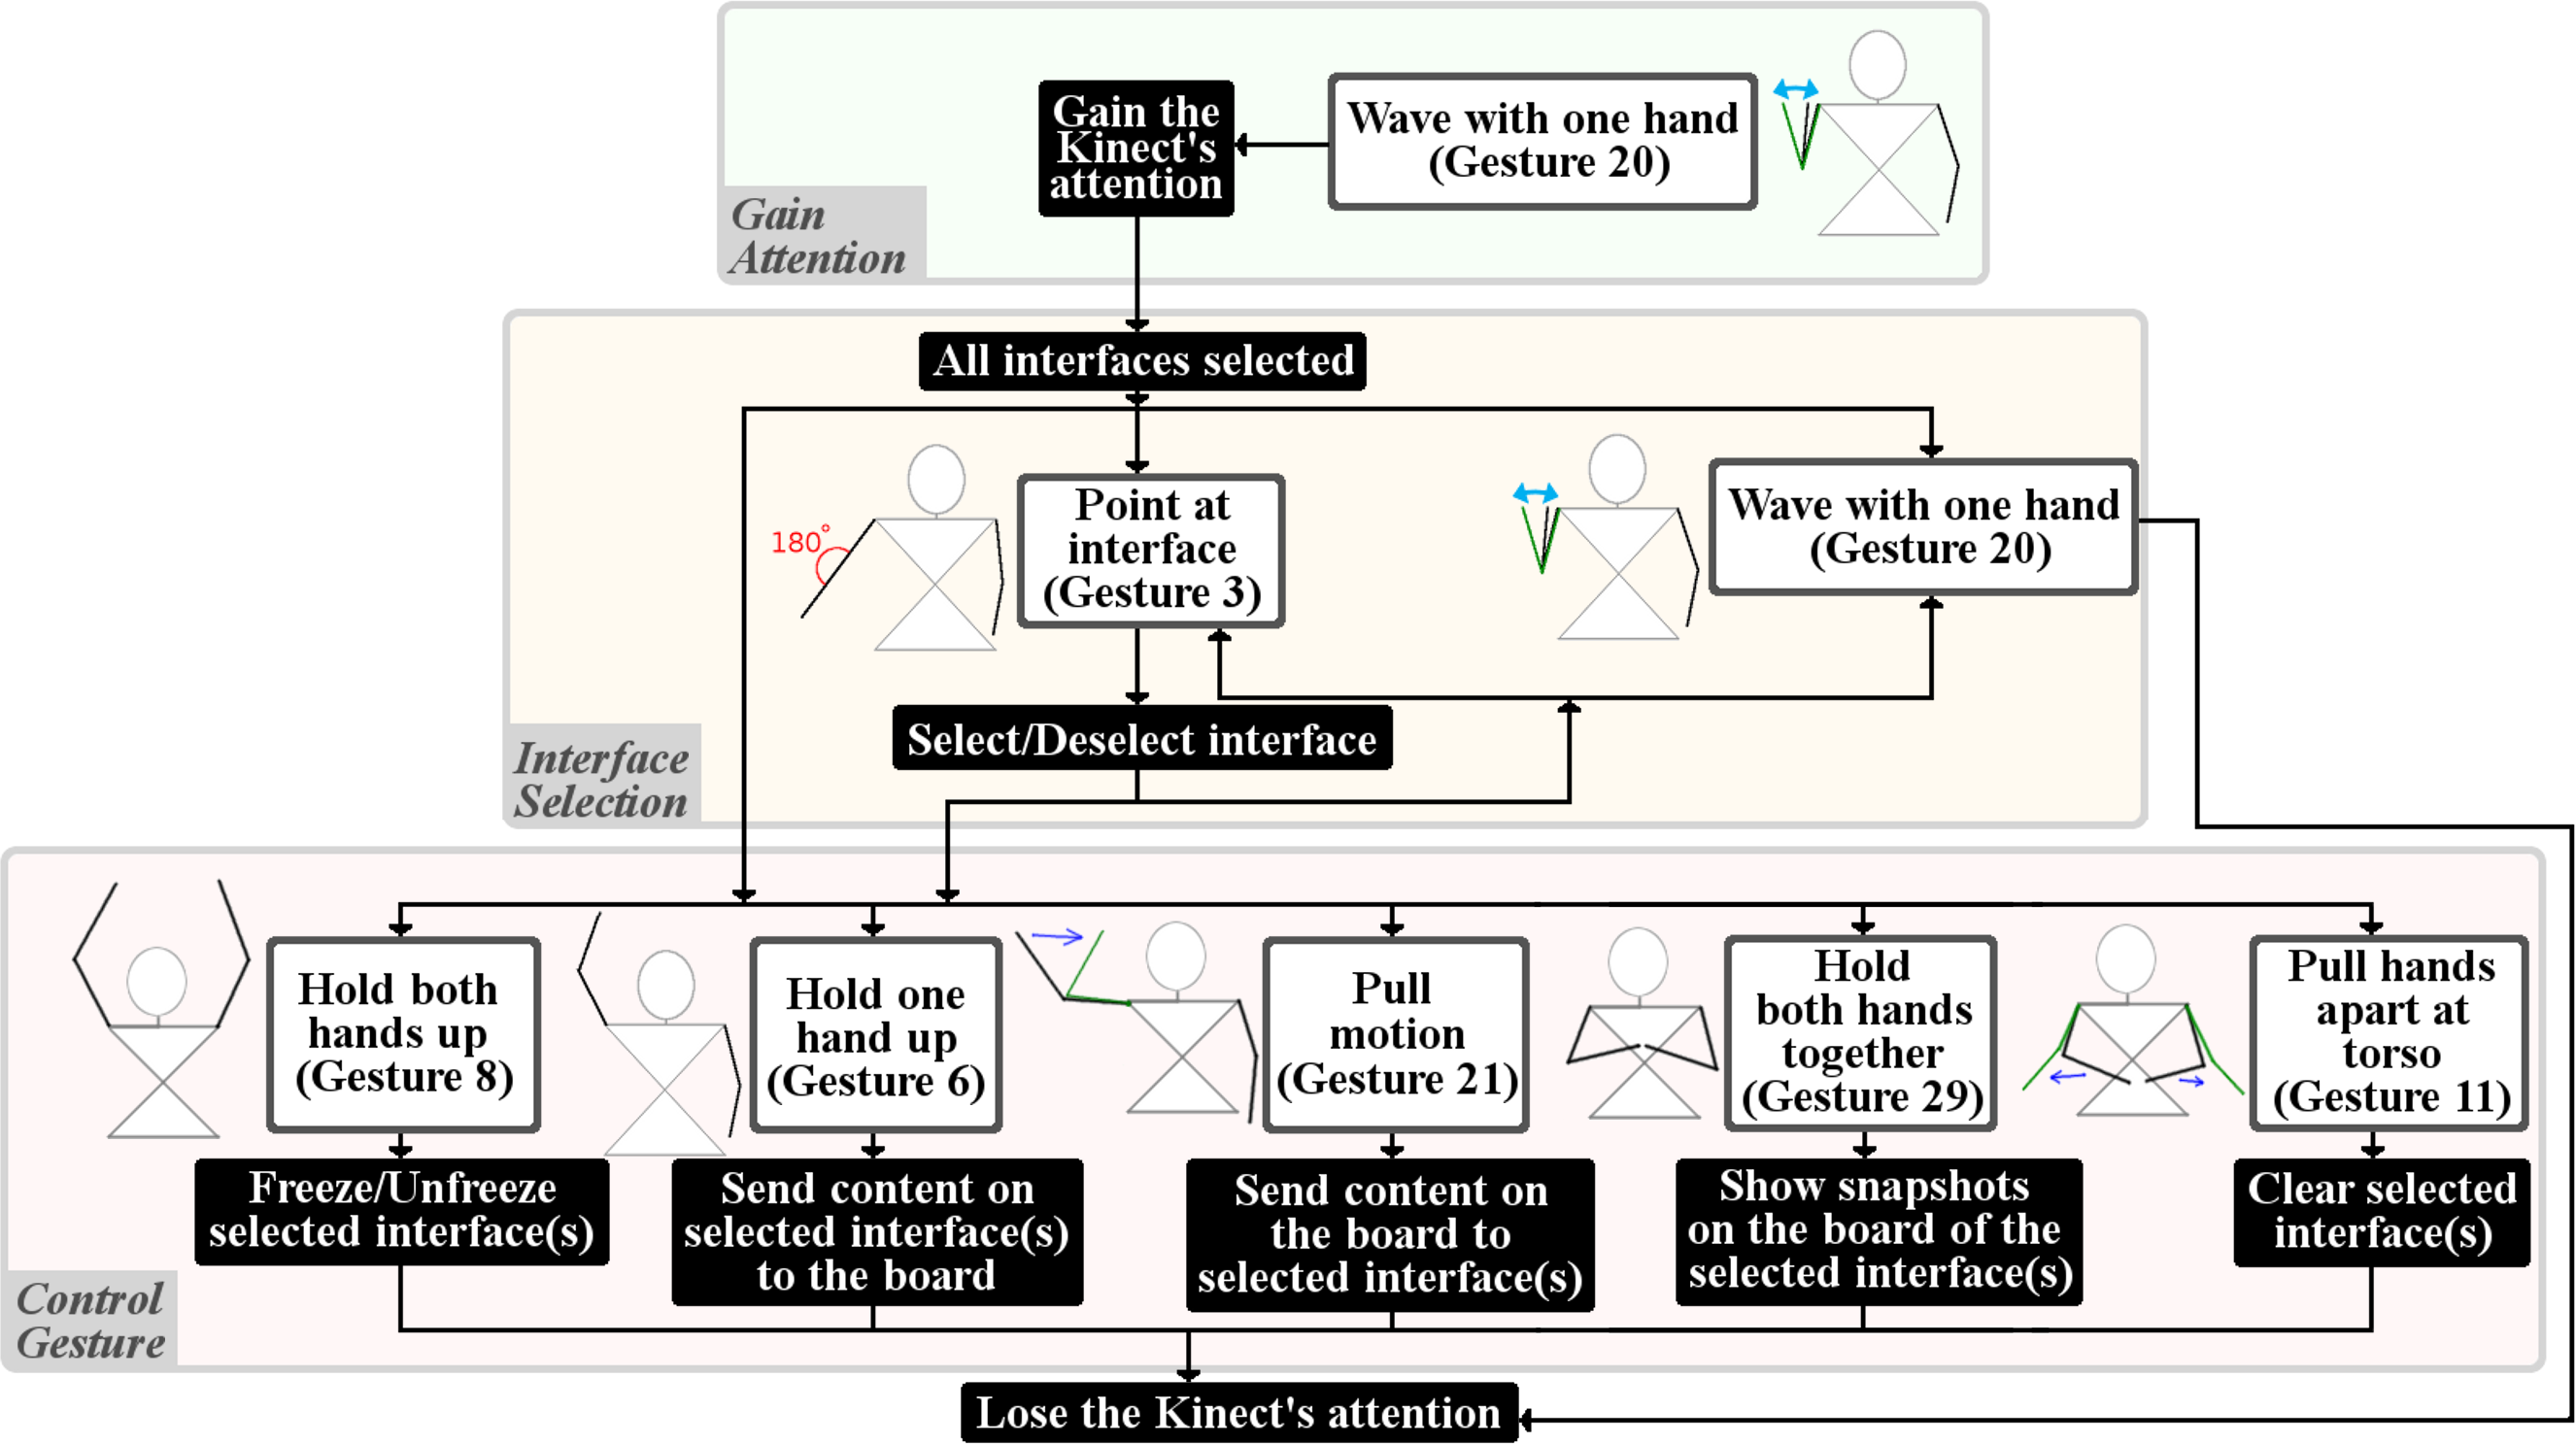
\includegraphics[width=1\textwidth]{figures/control_flow.png}
   \caption{How the gesture identified in the focus group are intended to be used.}
   \label{fig:flow}
\end{figure*}

Figure~\ref{fig:flow} outlines a control sequence in which the gestures and approaches to interface selection indicated by the focus group to be intuitive can be used to issue common commands to classroom technologies.
Teachers first obtain the light-coding device's attention with a wave then point to the interfaces they wish the following command gesture to affect.
The teacher can repeatedly point to interfaces to select and deselect them until they perform the command gesture.
Alternatively, the teacher can perform the command gesture immediately after obtaining the light-coding device's attention to issue the corresponding command to all interfaces.
At any time during this control sequence a teacher can wave again to dismiss the light-coding device's attention.
After the command gesture is performed the light-coding device stops paying attention to the teacher.

For each response of the system to teacher gestures, denoted in Figure~\ref{fig:flow} with the black boxes with white text, some form of feedback will need to be provided to the teacher.
This feedback is necessary for informing the teacher whether the gesture they have performed has had the intended effect on the system or not.

With the gesture set and control sequence defined, a classroom technology system can be augmented to use a light-coding device.

\section{Pilot Study}
\label{sec:pilotStudy}

To explore the suitability of the defined gesture set to use with a light-coding device it was decided that a pilot study was needed.
This pilot study would allow for any short-comings in the technology or gesture-set to be identified and corrected before carrying out any further studies.

\subsection{Software Implementation}
\label{subsec:pilotStudyImplementation}

The SynergyNet framework~\cite{Higgins2011} was selected for implementing the control sequence defined in Section~\ref{sec:background} into.
SynergyNet is a software framework which supports education based activities that are intended to be interacted with through multi-touch table interfaces.
The framework offers a wide range of supporting features such as communication between multiple interfaces via a network and is capable of displaying several forms of media.
SynergyNet accepts inputs from a range of multi-touch protocols, such as TUIO~\cite{Kaltenbrunner2009}.
Though initially intended for use with diffused illumination multi-touch technology~\cite{Matsushita1997}, the support of multiple protocols allows the framework to be used with a wide range of natural user input interfaces including interactive whiteboards and multi-touch tables.

Applications for SynergyNet often utilise the network functionality of the framework to allow teachers to orchestrate classroom activities.
Previously, teachers have been able to do this through a static multi-touch device~\cite{AlAgha2010}.
Teachers can also orchestrate SynergyNet through a web interface which can be accessed through a mobile touch device, such as a phone or tablet~\cite{Mercier2013}.
In previous studies using the SynergyNet framework it was noted that the use of both the static teacher console and mobile devices to issue commands distracted the teacher from the students whenever used~\cite{Hatch2011,Mercier2013}.
This often disrupted conversations between the teacher and students.

The SynergyNet framework may benefit greatly from the use of upper-body gestures. 
The commands chosen to find gestures for in the study were based on those used in the existing SynergyNet controls. 
Several commands facilitated by these controls involve sharing materials between student interfaces and the classroom's board; a large, wall mounted interface used to display content to a class.
These commands have been observed in previous studies of SynergyNet to be essential for orchestrating tasks across the system.

To support the implementation of the gesture control sequence a light-coding device was required.
The Microsoft Kinect (1st generation) light-coding device was chosen due to its low cost and availability.

\begin{figure}[h]
   \centering
   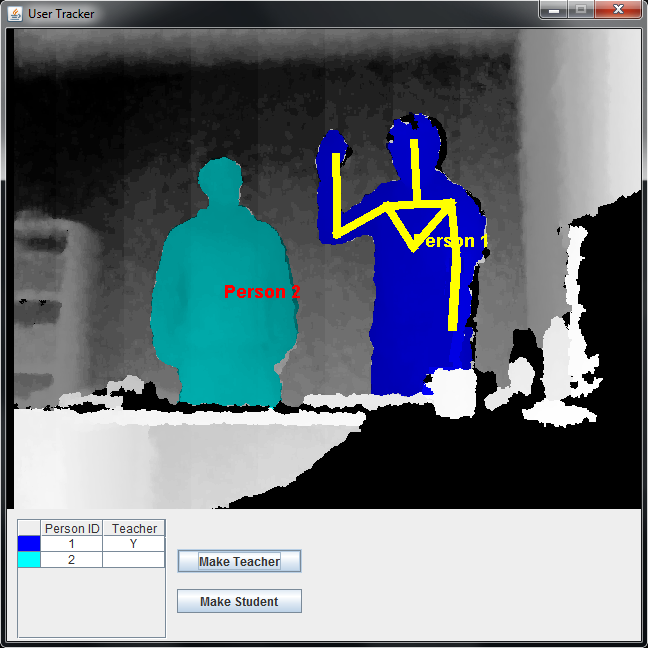
\includegraphics[width=0.45\textwidth]{figures/kinect_node.png}
   \caption{SynergyNet's Kinect node.}
   \label{fig:kinectNode}
\end{figure}

To integrate the Kinect with SynergyNet, the SensorKinect driver~\cite{Avin2011}, OpenNI library and NITE framework~\cite{OpenNi2021} were used together~\cite{Davison2012}.
Instances of SynergyNet running on the same network act as nodes which communicate through Hazelcast~\cite{Hazelcast2009}.
There are several different types of node used by SynergyNet defined by what device they as used on such as student-centric touch-screens or teacher control consoles.
For the implementation of the Kinect a new type of node was created which would manage tracking users, identifing gestures and displaying its current output, as shown in Figure~\ref{fig:kinectNode}.

The Kinect node obtains information on user locations relative to the sensor device position direct from the OpenNI framework.
Prior to use all SynergyNet nodes, including the Kinect node, will be configured so that it knows its associated device's position and orientation in the environment.
Before transmitting a tracked user's locational information, the Kinect node will use the knowledge of the sensing device's position to transform the locational information regarding the user to derive positions relative to the environment.

The Kinect node is used to identify when specific gestures are performed by a teacher.
When a teacher is observed performing a gesture the corresponding command is sent through the network to the relevant SynergyNet nodes.
The Kinect node has on-screen controls which allow identified persons to be designated as students or teachers, as shown in Figure~\ref{fig:kinectNode}.

Support for multiple Kinect devices was not possible in this pilot due to issues surrounding how the device's depth-detection techniques would interfere with other Kinect devices nearby~\cite{Maimone2012,Schroder2011}.
This meant that the use of the pointing gesture outlined in Section~\ref{subsec:userGeneratedGestures}'s defined control sequence used for selecting interfaces could not be implemented into SynergyNet.
For the pilot study it was decided that any commands issued through gestures would have to affect all student interfaces.

To minimise the potential of a false positive, a timer was implemented into the control sequence which would dismiss the Kinect's attention if no valid gestures are detected.
Once a teacher has waved and gained the attention of the Kinect they would have thirty seconds to perform a gesture in the control sequence.
Otherwise, the control sequence ends and the Kinect's attention is dismissed.
This ensured that if a teacher unknowingly gains the attention of the Kinect, the amount of time they could perform a gesture accidentally in is limited.

As discussed in Section~\ref{subsec:userGeneratedGestures}, the system needs to provide feedback to the teacher for each action of the system denoted in Figure~\ref{fig:flow}.
As part of the control sequence a sound was played when the Kinect's attention is gained to alert teachers of successful intentional or accidental unintentional waving gestures.
The use of audible feedback allows the teacher to be informed of this event without the need to focus on a visual output.
A visual form of feedback was also offered due to the potential problem of audio with ambient classroom noise as discussed in Section~\ref{sec:background}.
This visual feedback took the form of a border appearing on the Kinect node display.
A border also appears on all the student interfaces at this stage to indicate they are awaiting a command gesture.
This increases the chance of the teacher seeing the feedback informing them that they have successfully gained the Kinect's attention.

For the actions resulting directly from a command gesture the teacher can visually see the effect of the completed action as a form of feedback.
The movement and removal of content is clear enough that no additional feedback is required.
For the freezing and unfreezing of the system a blue tint is applied to the student interfaces in adherence to the metaphor of its content being frozen.

When the control sequence is finished the borders are removed from the Kinect node and student interface to indicate that the system's attention is lost.

\subsection{Pilot Study Design}
\label{subsec:pilotStudyDesign}

It was decided that the pilot study should be conducted as an observed lab-based experiment to discover what issues an full study might encounter with the implementation.
The study took place in the SynergyNet lab used in the focus group discussed in Section~\ref{subsec:focusGroupDesign}.
The objective of this pilot study was to find how usable the implementation of the upper-body gestures control system was.

The head teacher from a local school was chosen for participation in this study through convenience sampling.
A class of 12 of teacher's students who the teacher had taught previously also participated.
This class consisted of eight girls and four boys aged eight to ten.
The participating teacher was first given an hour long training session where they were brought into the SynergyNet system and lab.  

Following the training session, the teacher's class of students were introduced to the classroom.
The students were given the chance to gain familiarity with the multi-touch tables through interacting with several simple SynergyNet applications.
Following this the class then started the first \textit{mysteries} task.
Mysteries are a pedagogic technique, designed to support collaborative problem solving~\cite{Leat2002}.
The mysteries task gives groups of students a selection of clues relating to a particular scenario~\cite{Higgins2011b}.
Students are then given a question which they must use the clues to answer.
The task was chosen due to its requirement for the teacher to perform all the commands outlined in Section~\ref{subsec:userGeneratedGestures} throughout~\cite{Mercier2012}.
Before using the Kinect for orchestrating the classroom the teacher carried out several mysteries tasks with more traditional SynergyNet control devices, specifically the a large interactive board and a web interface on a tablet device.
This was to provide a background of typical usage to compare the use of the Kinect with.
Each of the mysteries tasks used different content but were of the same complexity.  

The teacher was asked to think aloud when possible and announce their intentions before executing a command.  
This allowed for timing of intention to execution and would allow for identification of unintended results.

\subsection{Pilot Study Results}
\label{subsec:pilotStudyResults}

\begin{figure}[h]
	\centering
   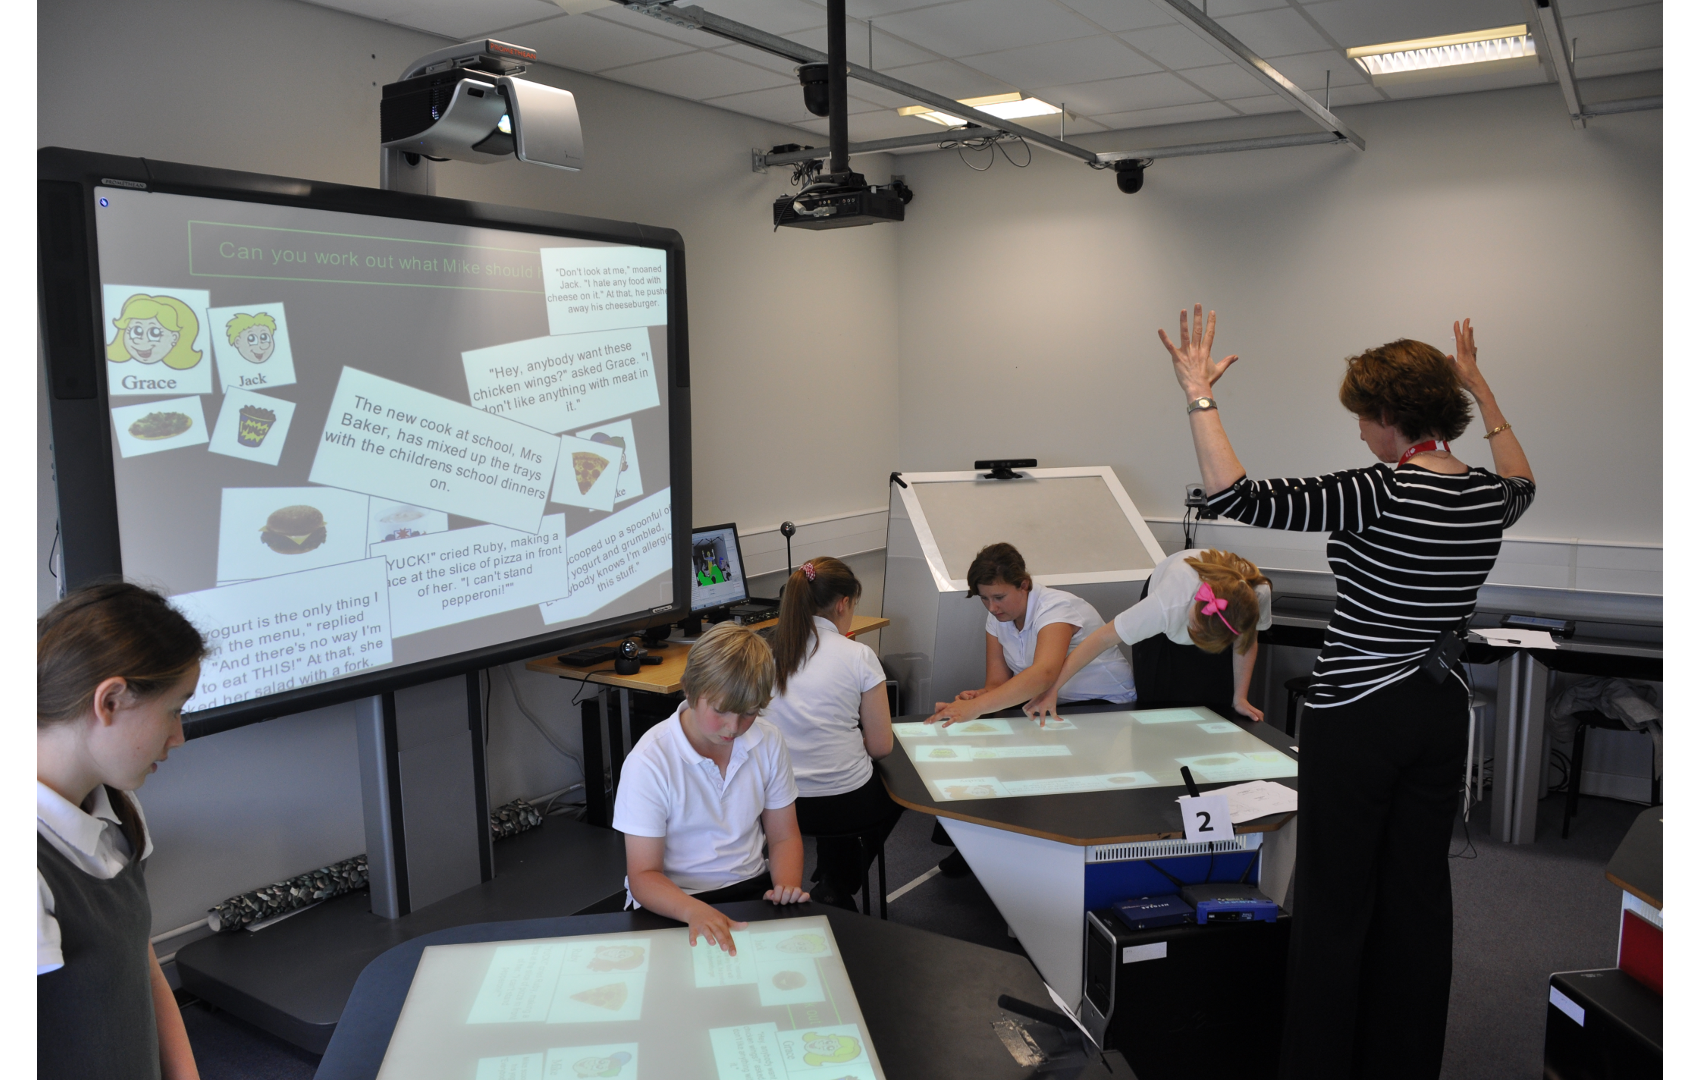
\includegraphics[width=0.45\textwidth]{figures/pilot_study_kinect.png}
   \caption{The Kinect device in use during the pilot study.}
   \label{fig:pilotStudyKinect}
\end{figure} 

For commands issued with the large interactive board:
\begin{itemize}
   \item The average time taken to issue a command was 12.5 seconds with a standard deviation of 6.36 seconds.
   \item 1/10 of the commands issued was erroneous.
\end{itemize}

For commands issued with the web interface through a tablet:
\begin{itemize}
   \item The average time taken to issue a command was 13.6 seconds with a standard deviation of 11.7 seconds.
   \item 1/9 of the commands issued was erroneous.
\end{itemize}

The average time taken to issue a command with the Kinect, as shown in Figure~\ref{fig:pilotStudyKinect}, was 6.6 seconds with a standard deviation of 5.59 seconds.
Of the twenty one commands issued during this task with the Kinect, eighteen were erroneous.

Six of these errors were caused by the teacher waving too many times.
This resulted in their third wave being interpreted as a command gesture.
The third wave was frequently interpreted as a pull gesture, which informs all the student-centric interfaces to show content on the board.
These false positives are the result of the control sequence being too easy to deviate from since in its implementation in the pilot it would expect specifically two waves.

Four of the errors were caused by the Kinect losing track of one of the teacher's hand.
Due to this, only one hand is identified as being above the teacher's head when in fact both are in the air.
This results in the gesture for the freeze command being interpreted as the gesture for sending content to the board.
These errors are the result of technical failures, caused by the limitations of the Kinect.

Two of the errors observed when using the Kinect were caused by the teacher trying to send contents to the tables when there was no content on the board to send.
These errors are attributed to user-error.

Two of the errors were caused by the teacher performing a gesture before getting the Kinect's attention.
These false negatives were caused by the teacher forgetting the control sequence.

A teacher pausing for a relatively long time between getting the Kinect's attention and performing a gesture was the cause of one of the errors observed during this task.
The Kinect's attention is configured to expire if a teacher takes too long to perform a gesture.
As the teacher was made aware of the time-out mechanism beforehand, this false negative can be interpreted as an error caused by the teacher not following the control sequence.
The control sequence could be improved to accommodate for longer pauses by the teacher.

One of the erroneous commands was caused by the teacher intending to perform a freeze gesture.
The Kinect saw the movement of the hands moving from torso out from the wave gesture to get attention and interpreted it as the gesture for clearing the student interfaces.
This false positive results from a fault in the control sequence design.

Another observed error was caused by the teacher pausing in the middle of a gesture.
Without movement the Kinect saw the teacher performing a pose which issued a different command.
The cause of this false positive was the teacher failing to follow the control sequence since pausing during the gesture was equivalent to performing a different gesture in the view of the Kinect.

A single error was caused by the teacher performing the wrong gesture.
The teacher intended to freeze the tables but performed the pull content gesture instead. 
This error was caused by the teacher making a mistake.
This may indicate that the gestures are not intuitive and can lead to confusion.
The teacher had performed the pull gesture for retrieving the content from the board immediately before committing this error.
Repeating the first part of the control sequence; waving, may have led to them continuing with the same actions without realising the need to change the command gesture.

The Kinect was noted to have experienced several issues which may account for the observed errors in the command sequence.
The Kinect lost track of the teacher's calibration three times.
In addition to this, the teacher presence was lost entirely by the Kinect three times.
This was potentially due to the Kinect's view of the teacher being partially obscured by students moving about the tabletop interfaces.

The teacher spent a significant amount of time trying to unfreeze the tables.
The repeated errors prolonged this process which would usually require a single command.
Due to the high number of errors caused by the Kinect, students became frustrated.
There appeared to be two causes of the majority of the errors:

\begin{itemize}
\item The teacher was waving too much when obtaining the Kinect's attention.
\item The Kinect repeatedly lost track of the teacher and their limbs. 
\end{itemize}

Three of the errors noted during this task could be categorised as false negatives whereas eight of the errors were false positives.

\subsection{Pilot Study Observations}
\label{subsec:pilotdiscussion}

Several shortcomings of the Kinect became evident throughout the pilot study.

The first potentially stemmed from the training of the teacher participating.
The one hour training may not have been enough time to allow the teacher to gain familiarity with the control devices.
This may have contributed a number of failures to follow the command sequences, especially with the Kinect.

The Kinect encountered several technical issues throughout the pilot study which prevented it from accurately tracking the teacher, their limbs and their joints.
This inability to track could have been caused by the teacher leaving the Kinect's field of view.
The classroom environment set up in the lab was larger than the Kinect's range.
Due to this, the teacher often wandered beyond the Kinect's range to monitor and talk to students positioned around the distant tabletop interfaces.
Whenever the teacher travelled outside the Kinect's field of view for more than several seconds the Kinect would lose track of their calibration and identity.
This meant that if the teacher did not establish their teacher status on re-emerging into the Kinect's view then their subsequent gestures were not recognised.
It is important to note that the Kinect's range is limited to three and a half metres~\cite{Maimone2011} and a sixty degree viewing angle~\cite{Stone2011}, this covers most of the area in the lab used in the pilot study (which is designed to be the same size as an average classroom) but not all.

Even when the teacher stayed within the Kinect's field of view, technical issues relating to the device's range caused errors.
If the teacher was positioned close to the limits of the Kinect's range performing gestures, the device's limb and joint tracking became inaccurate.
This is a known limitation of the device~\cite{Mehrotra2011}.
The device would often lose track of the teacher's limbs and joints, seeing them either move erratically or appear at rest when in fact the teacher was moving them to perform a gesture.
When a limb was obscured the Kinect would attempt to position it, often resulting in an inaccurate placement.
This also led to the limb positions moving erratically which caused several of the errors in the gesture recognition system.

A number of the errors that occurred when using the Kinect were established to be caused by the design and implementation of the control sequence.
The majority of these relate to the movement of hands immediately after obtaining the Kinect's attention.
The movement of the teacher's hands when finishing the attention-grabbing wave gesture were on occasion interpreted as a separate command gesture.
In addition to this, the Kinect often interpreted the movement of hands to positions needed to perform a command gesture as the command gesture itself.

The pilot study has revealed four criteria~\cite{Wachs2011} in which SynergyNet's upper-body gesture controls needs improvement; 
\textit{accuracy}, \textit{interaction space}, \textit{intuitiveness} and \textit{mental load}.
It is possible to summarise the issues which resulted in the system being incapable of meeting these three criteria as so:

\begin{itemize}
\item \textbf{Issue 1: Losing Track of Users, Limbs and Joints:}
This refers to errors caused by the teacher's leaving the accurately observable area of the Kinect devices.
\item \textbf{Issue 2: Gesture Confusion:}
This issue encompasses all errors caused by the teacher in the pilot study making mistakes by confusing or forgetting gestures.
\item \textbf{Issue 3: Stringent Control Sequence Requirements:}
This issue refers to errors encountered when the teacher accidentally deviated from the defined control sequence.
\item \textbf{Issue 4: Reduced Functionality:}
This relates to how the limitations of a single Kinect meant that a part of the control sequence defined in Section~\ref{subsec:userGeneratedGestures} could not be implemented.
\end{itemize}

The pilot study made it clear that these identified issues would need to be resolved as part of the implementation of the study.

\section{Resolving Issues Observed in Pilot Study}
\label{sec:resolvingIssuesObserved}

The issues outlined in the pilot study were noted to make the use of the system counter-productive.
The benefits afforded by the system of non-intrusive and quick command execution were made irrelevant due to the high number of errors caused by the identified issues.
Resolving these issues could allow the system to function as intended and would allow the potential benefits of the upper-body gesture controls to be evaluated and employed.

\subsection{Resolving Issue 1: Improving the System's Tracking}
\label{subsec:resolvingIssuesObserved1}

To improve the accuracy and monitored area of the sensing technology used with the system, multiple Kinects could be employed.
With more Kinect devices in the environment, more of the classroom would be monitored.
A larger monitored area reduces the chance of the teacher losing their calibrated status by wandering out of the Kinects' view.
This saves time by reducing how often the teacher needs to repeat the calibration process.

Dubois et al.~\cite{Dubois2011} track the movement of mobile objects through an apartment using two Kinects.
Using knowledge of the Kinects' positions relative to each other, their visual and depth information can be stitched together.
Any processing applied to the information provided by the Kinect to track the movement of mobile objects can then be applied to the combined output.
Stitching the information requires a large amount of processing power.
However, once done it allows for the later process-intensive functions used to identify and track mobile objects to be applied just once, rather than having separate process-pipelines for each Kinect.

Luber et al.~\cite{Luber2011} utilise multiple Kinects in their work to track persons across large environments.
Through a form of user recognition the system presented is able to track a person as they cross from one Kinect's field of view to another.
The system tracks the movement of persons across their viewed areas.
On the Kinect identifying a person the system determines their unique visual and geometric features.
Whenever a new person is identified on a Kinect the system checks to see if they have been seen before on another Kinect by comparing their features.
If so, then the system can then establish the movement of persons across multiple fields of view.
This allows for a person's movement to be tracked across a larger area.

Overlapping the views of the Kinects would eliminate the need for teacher's to perform gestures towards the limits of a single Kinect's view.
This ensures that teachers stay within the areas of the Kinects' view which are more accurate.
However, when the views of two or more Kinects overlap there is the potential issue of interference~\cite{Satyavolu2012}.
The two multiple Kinect systems discussed so far~\cite{Dubois2011,Luber2011} avoid this issue by ensuring that the overlapping area of Kinect views is minimised.
The Kinect functions by projecting a pattern of infra-red light.
Because all Kinect devices produce, and look for, this light pattern at the same frequency it is possible for one Kinect device to see the pattern produced by another.
The Kinects cannot distinguish the infra-red light patterns and will interpret the pattern from another Kinect as its own.
The Kinect uses deformations in their projected pattern to detect the placement of objects.
If two patterns overlap the Kinect will not be capable of accurately identifying these deformations and their implications.
This interference can significantly reduce the accuracy of Kinect devices~\cite{Satyavolu2012}.

To avoid multiple Kinects viewing each other's patterns, the sensing devices can be positioned in perpendicular planes~\cite{Caon2011,Kramer2012}.
Positioned ninety degrees from another Kinect ensures that it will not view any of the infra-red light projected direct from the other device.
This positioning will also minimise the amount of infra-red light the Kinect sees from the surfaces the other device's pattern is projected onto.
This reduces interference to a level where the Kinect is capable of accurately tracking persons' limbs and joints~\cite{Caon2011}.
The setup used by Dubois et al.~\cite{Dubois2011} also entails positioning the two Kinects used perpendicular to each other so that either Kinect cannot see the other's projected pattern.
This approach does increase the accurately monitored area of a system of Kinect devices but does have a restriction; only two Kinects can have overlapping views.
If more than two Kinects are positioned perpendicular to its neighbours then at least two of the devices will be in parallel.
This means that the two parallel devices' will interfere with each other, reducing their accuracy.

A potential technique of using multiple Kinects together without their projected patterns interfering with each other is time division~\cite{Schroder2011}.
This is where the Kinects in a system will take it in turns to project and view their patterns.
Any pairing of Kinects which cause interference can be set up so that they never project at the same time.
However, a Kinect will not be collecting any usable depth information while another Kinect which could interfere with it is projecting.
Due to this,  the technique causes a reduction in the frame-rate of the depth image collected from the devices.
The accuracy of the devices afforded by removing interference is traded-off for a reduction in responsiveness.
Therefore, the adoption of this technique, while resolving the issue of accuracy may result in the system being unable to meet the criteria for responsiveness.

Another potential technique for reducing the interference caused by overlapping light patterns is the movement of the sensing devices~\cite{Maimone2012}.
By moving a Kinect, the device's projected pattern is moved along with its camera.
If no other device is currently performing the same motion the system should be capable of identifying the reflected light from a unique Kinect.
This has been shown to reduce interference when multiple Kinects are used together~\cite{Maimone2012} but does have the requisite that the devices are constantly in motion.
Large movements which change the Kinects' locations may complicate any calculations which utilise the positional information provided by the devices.
Constant movement of the devices would require additional calculations to transform the relative positional information output from a Kinect to their real-world locations.
This additional calculation could reduce the system's responsiveness.
Vibration of the Kinect could be used to minimise the movement required to differentiate the devices' projected patterns~\cite{Kainz2012}.
However, to add any motion to the Kinect devices, extra cost must be spent to implement the motors needed to automate this movement.
The adoption of this technique, while resolving the issues relating to accuracy and interaction space, may result in the system being unable to meet the criteria for cost.

To differentiate the infra-red light produced and received by the Kinect devices, filters could be employed.
Multiple depth-cameras using the same structured light setup as the Kinect have been made capable of working together through filtering the infra-red used~\cite{Kim2008}.
However, the Kinect is not capable of this~\cite{Kainz2012}.
The Kinect produces and views a very small range of infra-red frequencies.
Filtering this would reduce the range of frequencies visible to each Kinect further and would likely result in the depth image becoming more inaccurate.

The techniques discussed so far for allowing multiple Kinect devices to work together involve providing methods of differentiating the devices' projected light patterns.
Wang et al.~\cite{Wang2012} present a potential technique which reduces the influence of interference caused by multiple Kinects not through prevention but correction.
The technique uses the depth information collected from the devices to reconstruct the scene viewed.
In areas where the depth information is missing due to interference, a plane-sweeping based algorithm is used to regenerate the lost information.
The algorithm uses the existing depth data from all the Kinect devices to calculate the missing information.
The initial results shown from Wang et al.'s~\cite{Wang2012} simulations are promising but there may be issues with using this technique in a real-world scenario.
The time and processing power required by the algorithm could reduce the system's responsiveness.

It should be possible to use the gesture control sequence devised in the guessability study with an alternative depth sensing technology~\cite{Kean2011}.
These alternatives may resolve the issues relating to accuracy and interaction space but could incur other issues.
The Primesense~\cite{Wilson2010} depth camera performs the same function as the Kinect and could be used with SynergyNet.
However, the device uses the same structured light technique as the Kinect meaning the same issue of interference would likely still be present.
Oblong's Mezzanine~\cite{kramer2011} uses custom built depth cameras to observe user's movement in a meeting room environment.
The system's range is greater than that of a single Kinect but its cost far exceeds that of several of Microsoft's devices.
Wearable devices could be used for tracking gestures more accurately than the Kinect~\cite{Rekimotoa,Zhu2011}.
However, improved accuracy these device may not outweigh the un-encumbering benefits of a technology like the Kinect.

\subsection{Resolving Issue 2: Improving Gestures}
\label{subsec:resolvingIssuesObserved2}

To improve the intuitiveness of the SynergyNet upper-body gesture system it is possible that a number of the gestures may need to be changed.
The pilot study highlighted the issue with gestures that do not relate to real-world actions. 
The waving and holding of one hand up are the only gestures in the set which bear no relation to related real-world actions.
Changing these gestures to ones resembling related real-world actions may improve their intuitiveness.

It is possible that many of the errors committed in the pilot study may have been avoided if the teacher participating had better training with the system.
In the pilot study the teacher had a single hour to learn how to use SynergyNet.
It is possible that this may not have been enough time for the teacher to gain sufficient confidence with using the system.
Giving the teacher more time for training may make their use of the system less error-prone.

\subsection{Resolving Issue 3: Improving the Control Sequence}
\label{subsec:resolvingIssuesObserved3}

In the pilot study, the teacher participating often committed errors due to following the command sequence incorrectly.
Many of these errors were due to the teacher stopping to think about the next gesture to perform in the command sequence.
One solution to this issue could be to reduce the time teachers spend recalling the next gesture they need to perform.
A more cohesive gesture set may reduce mental load and decrease the time taken for this.

The issues caused by the teacher pausing to think could also be resolved by making the control sequence more tolerant.
By allowing the control sequence to anticipate the user pausing the pauses will not necessarily be interpreted as a gesture.
In addition to this, enabling the system to anticipate and ignore movement between gestures during the control sequence will eliminate errors relating to the wrongful identification of unintended gestures.

Due to the issues with accuracy and interaction space, the Kinect often lost track of the teacher and their limbs in the pilot study.
This required the teacher to repeat the calibration pose several times and subsequently complicated the control sequence.
Improvements to the sensing system's accuracy and interaction space may also resolve issues related to mental load by reducing the number of times the calibration process needs to be repeated.
Automation of the calibration process may also simplify the control sequence.
Several Kinect-supporting frameworks, such as OpenNI~\cite{OpenNi2021}, have developed support for pose-less calibration where the Kinect is able to identify the joints and limbs of a person without the need for them to maintain a specific calibration pose.

User recognition may resolve issues related to mental load by reducing the amount of user intervention required for calibration.
The Kinect is capable of collecting biometric information on users it monitors from their appearance~\cite{Leyvand2011}.
Facial recognition, clothing colour tracking and height estimation can be used to distinguish monitored users.
This information can be stored and used when persons are viewed in the future to establish their identity.
User recognition, coupled with automatic calibration, would allow the system to calibrate the teacher with no user intervention after the teacher's identity is established.
This would allow the teacher to leave and re-enter the system's monitored environment on numerous occasions without needing to repeat any calibration steps.
This would reduce the amount of user intervention required by the control sequence.

\subsection{Resolving Issue 4: Adding Functionality}
\label{subsec:resolvingIssuesObserved4}

In the pilot study a method of selecting interfaces for a command to affect was not implemented.
The use of multiple sensing devices, as proposed for the resolution of issue 1 in Section~\ref{subsec:resolvingIssuesObserved1}, could allow the originally proposed pointing gesture to be implemented into the control sequence.
With multiple Kinects, when the teacher's body obscures the view of a Kinect when pointing, another of the devices should be able to see the obscured area and identify which interface is being pointed at.

\section{Study}
\label{sec:study}

With the potential solutions outlined in Section~\ref{sec:resolvingIssuesObserved} for the issues observed in the pilot study, a study could be carried out to assess the usage of the upper-body gesture control sequence derived in Section~\ref{subsec:userGeneratedGestures}.
It was a decided that the study should investigate how the control sequences compares with the use of more traditional methods of orchestrating technology in the classroom.
It was decided that the implementation created for the pilot study discussed in Section~\ref{sec:pilotStudy} could be built upon for this study utilising the suggested solutions to the pilot study issues.

\subsection{Software Implementation}
\label{subsec:studyImplementation}

With clear definitions of the issues in Section~\ref{subsec:pilotdiscussion} and their potential solutions in Section~\ref{sec:resolvingIssuesObserved}, improvements can be implemented in SynergyNet.
Five improvements were selected for implementation for the study.

\subsubsection{Multiple Kinects} 
\label{subsubsec:studyImplementationMultipleKinects}

It was decided that the SynergyNet system should be modified to allow for the use of multiple Kinects.
This was the most cost-effective way to improve the system's accuracy.
The use of multiple Kinects should also allow the devices to view teachers from multiple perspectives.
This reduces the issue of obstruction and as a consequence, improves the system's ubiquity.
This could also reduce mental load as the teacher will not need to put as much forethought into positioning themselves so that they are visible to a sensing device.

To avoid the issue of interference, noted in Section~\ref{subsec:resolvingIssuesObserved1} to occur when multiple Kinects are used together, the strategy of placing the devices perpendicular to each other was adopted.
This reduces interference and does not incur any additional cost.
This does, however, reduce the maximum number of Kinect devices which can be used together to two which is enough to cover the SynergyNet lab where the study would take place.

To combine the information collected from the Kinect devices a multiplexing approach was applied to the positional information they produce.
This was done through taking the user and joint location information from the devices and transforming them to be relative to the environment they exist within.
If two or more locational points supplied by different devices are noted to inhabit the same space the system determines that they are the same user or joint viewed by multiple devices.
This ensures that no duplication of locational information takes place and allows the system to identify when the same entity is seen by multiple devices.
This is similar to how touch information from multiple sources can be multiplexed together using the TUIO protocol~\cite{Kaltenbrunner2009}.
Through the use of multiplexing, SynergyNet is capable of tracking a user across the view of multiple Kinects as long as there is some overlap in the areas they monitor.
Therefore, a teacher should not need to re-establish their identity when moving about the environment.

A new SynergyNet node was created to support the act of collecting and combing information from multiple Kinect devices.
A single instance of this node, referred to as a multiplexer, is intended to run in the SynergyNet system, collecting information sent out by Kinect nodes.
The multiplexer can then distribute the locational information to other nodes.
The multiplexer node can identify which points of locational information from separate Kinect nodes are the same entity.

This multiplexing approach was chosen over alternatives, such as stitching the visual and depth views from the devices~\cite{Dubois2011}, due to its minimal processing costs.

\subsubsection{Gesture Set Cohesion} 
\label{subsubsec:studyImplementationGestureSet}

To improve the cohesion of the gesture set it was decided that all the upper-body gestures used in the control sequence should relate real-world actions as discussed in Section~\ref{subsec:resolvingIssuesObserved2}.
It was also noted that several of the gestures in the set did not follow this pattern.
Changing the gestures that did not relate to real-world actions to be more intuitive could reduce the mental load required by the control sequence as they act as metaphors~\cite{Wang2008}.

To identify the most suitable gestures to change the results from the original guessability study were revisited.
When ranking gestures by popularity amongst participants in the study this time, any gestures which do not resemble a related real-world action were discounted.
Two of the gestures in the existing gesture set were identified not to follow the metaphor pattern.

The holding up of one hand in the air, used to send content to the board, was identified as not conforming to a metaphor.
The gesture bares little to no resemblance to any real-world action involving sending or retrieving objects.
The highest ranking based gesture for the command of sending content to the board which conforms to being a metaphor was a pushing motion.
Therefore, it was decided this gesture would be used to replace the previously used one.
The suitability of the pushing gesture is supported by its resemblance to the pulling gesture used for the related command of retrieving content from the board.

The second gesture identified as not following the metaphor pattern was the waving gesture used to gain the Kinect's attention.
While waving is an action used to gain attention in most real-world scenarios it is more commonly used as a greeting and in UK classrooms the more common gesture for attracting attention is the holding up of one hand.
One of the most popular gestures in the study was the holding of one hand up.
With this gesture no longer being affiliated with the command to pull content from the board it was decided that it would be appropriate to repurpose it for gaining the Kinect's attention.

\subsubsection{Enabling Pause Tolerance}  
\label{subsubsec:studyImplementationPauseTolerance}

A pause was implemented into the control sequence before and after identifying a teacher performing a gesture.
These pauses are where the system will ignore any actions performed by the teacher, reducing the likelihood of unintentional gestures being performed.
These pauses last one and a half seconds, giving teachers time to move their limbs to the appropriate positions for the next gestures without significantly slowing down the control sequence.

\subsubsection{Automatic Calibration}  
\label{subsubsec:studyImplementationAutoCalibration}

The control sequence was also augmented by the implementation of automatic calibration.
This reduces the amount of input the teacher needs to provide into the control sequence, thus reducing the mental load required to operate the system.
The implementation of automatic calibration is also beneficial for the implementation of multiple Kinects, without it the teacher would be required to perform the calibration pose in front of each Kinect before use.

\subsubsection{Interface Selection}  
\label{subsubsec:studyImplementationInterfaceSelection}

The control sequence was augmented to include the pointing gesture for the selection of interfaces.
By pointing at an interface, the teacher can select the specific instances of SynergyNet to be affected.
Teachers can de-select an interface by pointing at it again.
If a teacher performs the command gesture without pointing at any interfaces, the corresponding command will affect all interfaces.

To identify a pointing gesture the Kinect node notes when the angle between a teachers upper and fore-arms at the elbow is close to one hundred and eighty degrees at the appropriate point in the control sequence.
If the arm is pointing directly down or up it is ignored as it is unlikely to be pointing to an interface.
When a pointing gesture is made, the vector along which the arm points and the location of the pointing hand relative to the environment are calculated.
The SynergyNet instance can then verify whether a ray fired along the pointing vector would intersect with a SynergyNet interface.
If so, this triggers a selection or de-selection event.

\begin{figure*}[t]
  \centering
  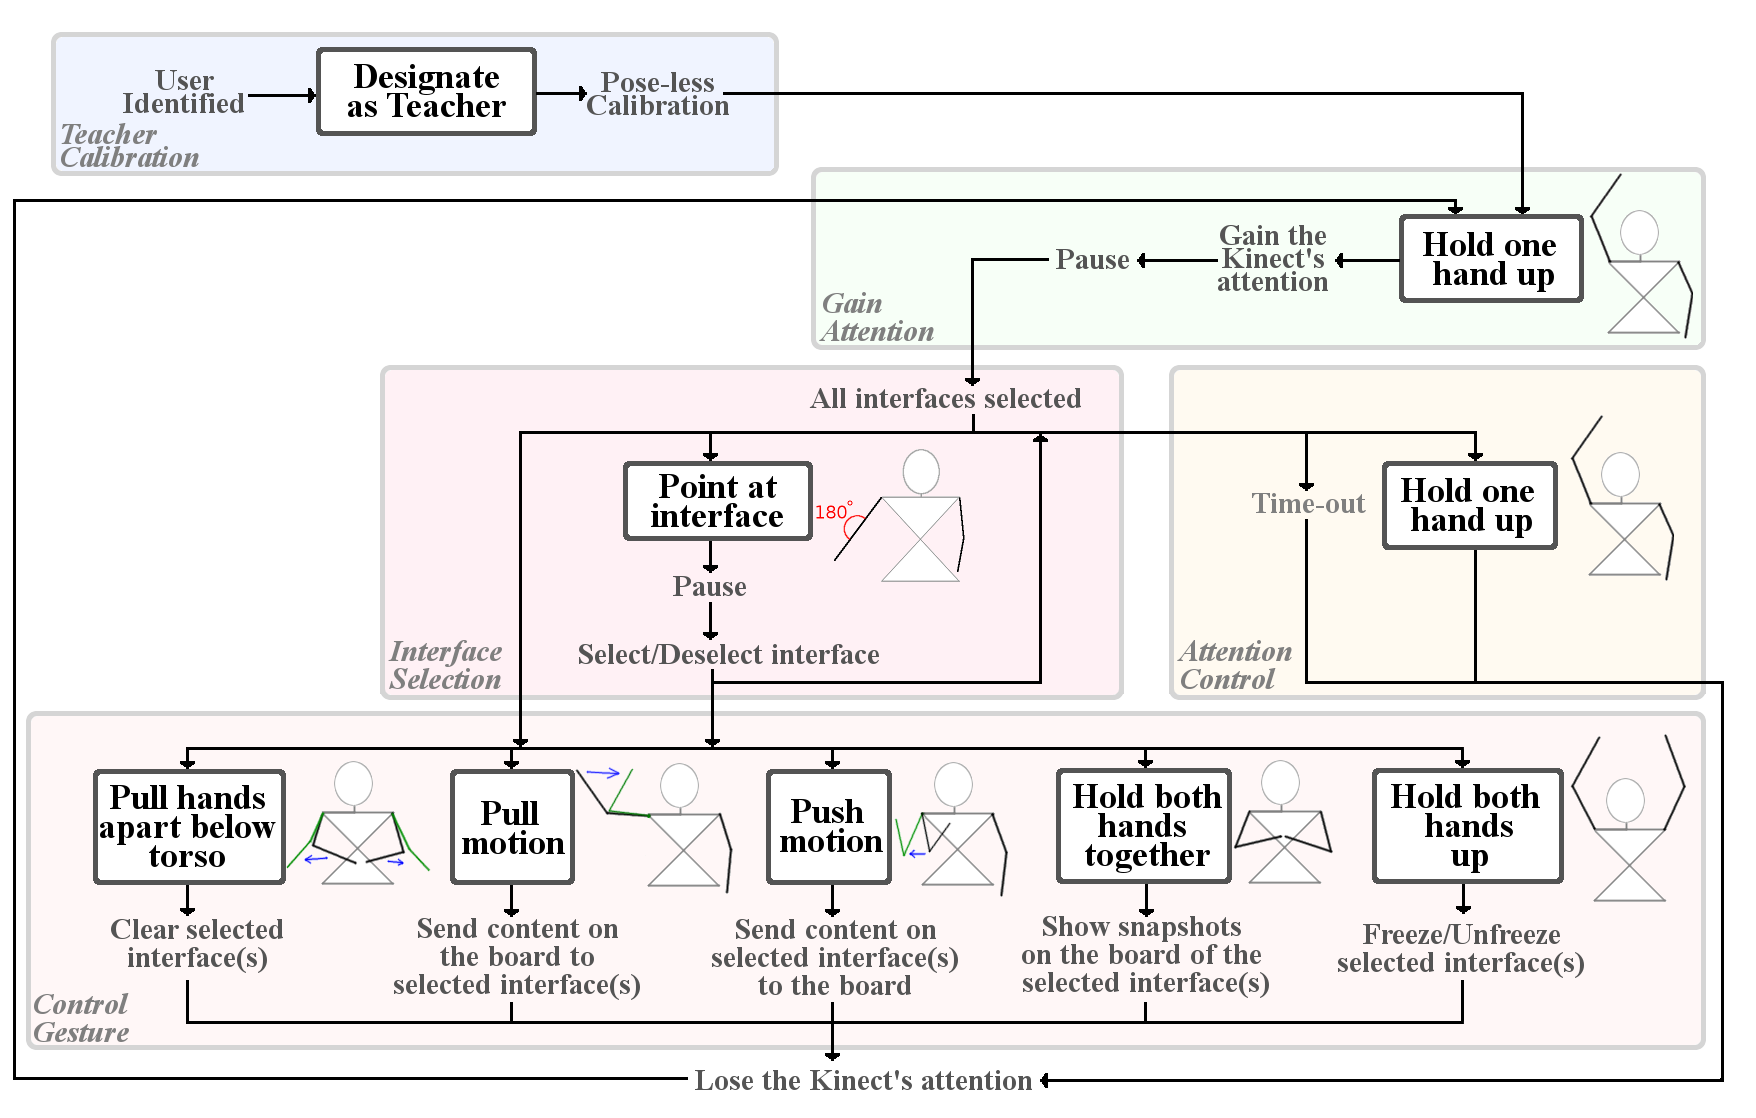
\includegraphics[width=1\textwidth]{figures/control_sequence_flow_diagram.png}
  \caption{The improved control sequence implemented for the gesture controls in SynergyNet.}
  \label{fig:controlSequenceFlowDiagram}
\end{figure*}

The updated control sequence with new gestures and interface selection is summarised in Figure~\ref{fig:controlSequenceFlowDiagram}.

\subsection{Design}
\label{subsec:studyDesign}

A study was organised to assess whether gestures are a viable method for controlling technology in the classroom.
A primary-school level teacher took part in the study with sixteen of their students.
The teacher was asked to orchestrate four \textit{mysteries} tasks~\cite{AlAgha2010} similar to those used in the pilot study.
For the first three tasks the teacher would use a single control technology; a large interactive whiteboard, a tablet or the Kinect, for issuing commands to the student interfaces.
For the final task teachers had all three technologies made available for their use.
The session was recorded for later data analysis.

The participating teacher was invited into the lab for a day in the week preceding their session.
On this day the teacher was introduced to the control technologies, given a chance to review the tasks to be performed and was allowed to carry out a dry-run of the session.
The teacher was encouraged to \lq think aloud\rq\ throughout the study and announce their intentions before issuing commands through a control technology.
Following the session the teacher was interviewed by the study organisers.

\begin{figure}[h]
  \centering
  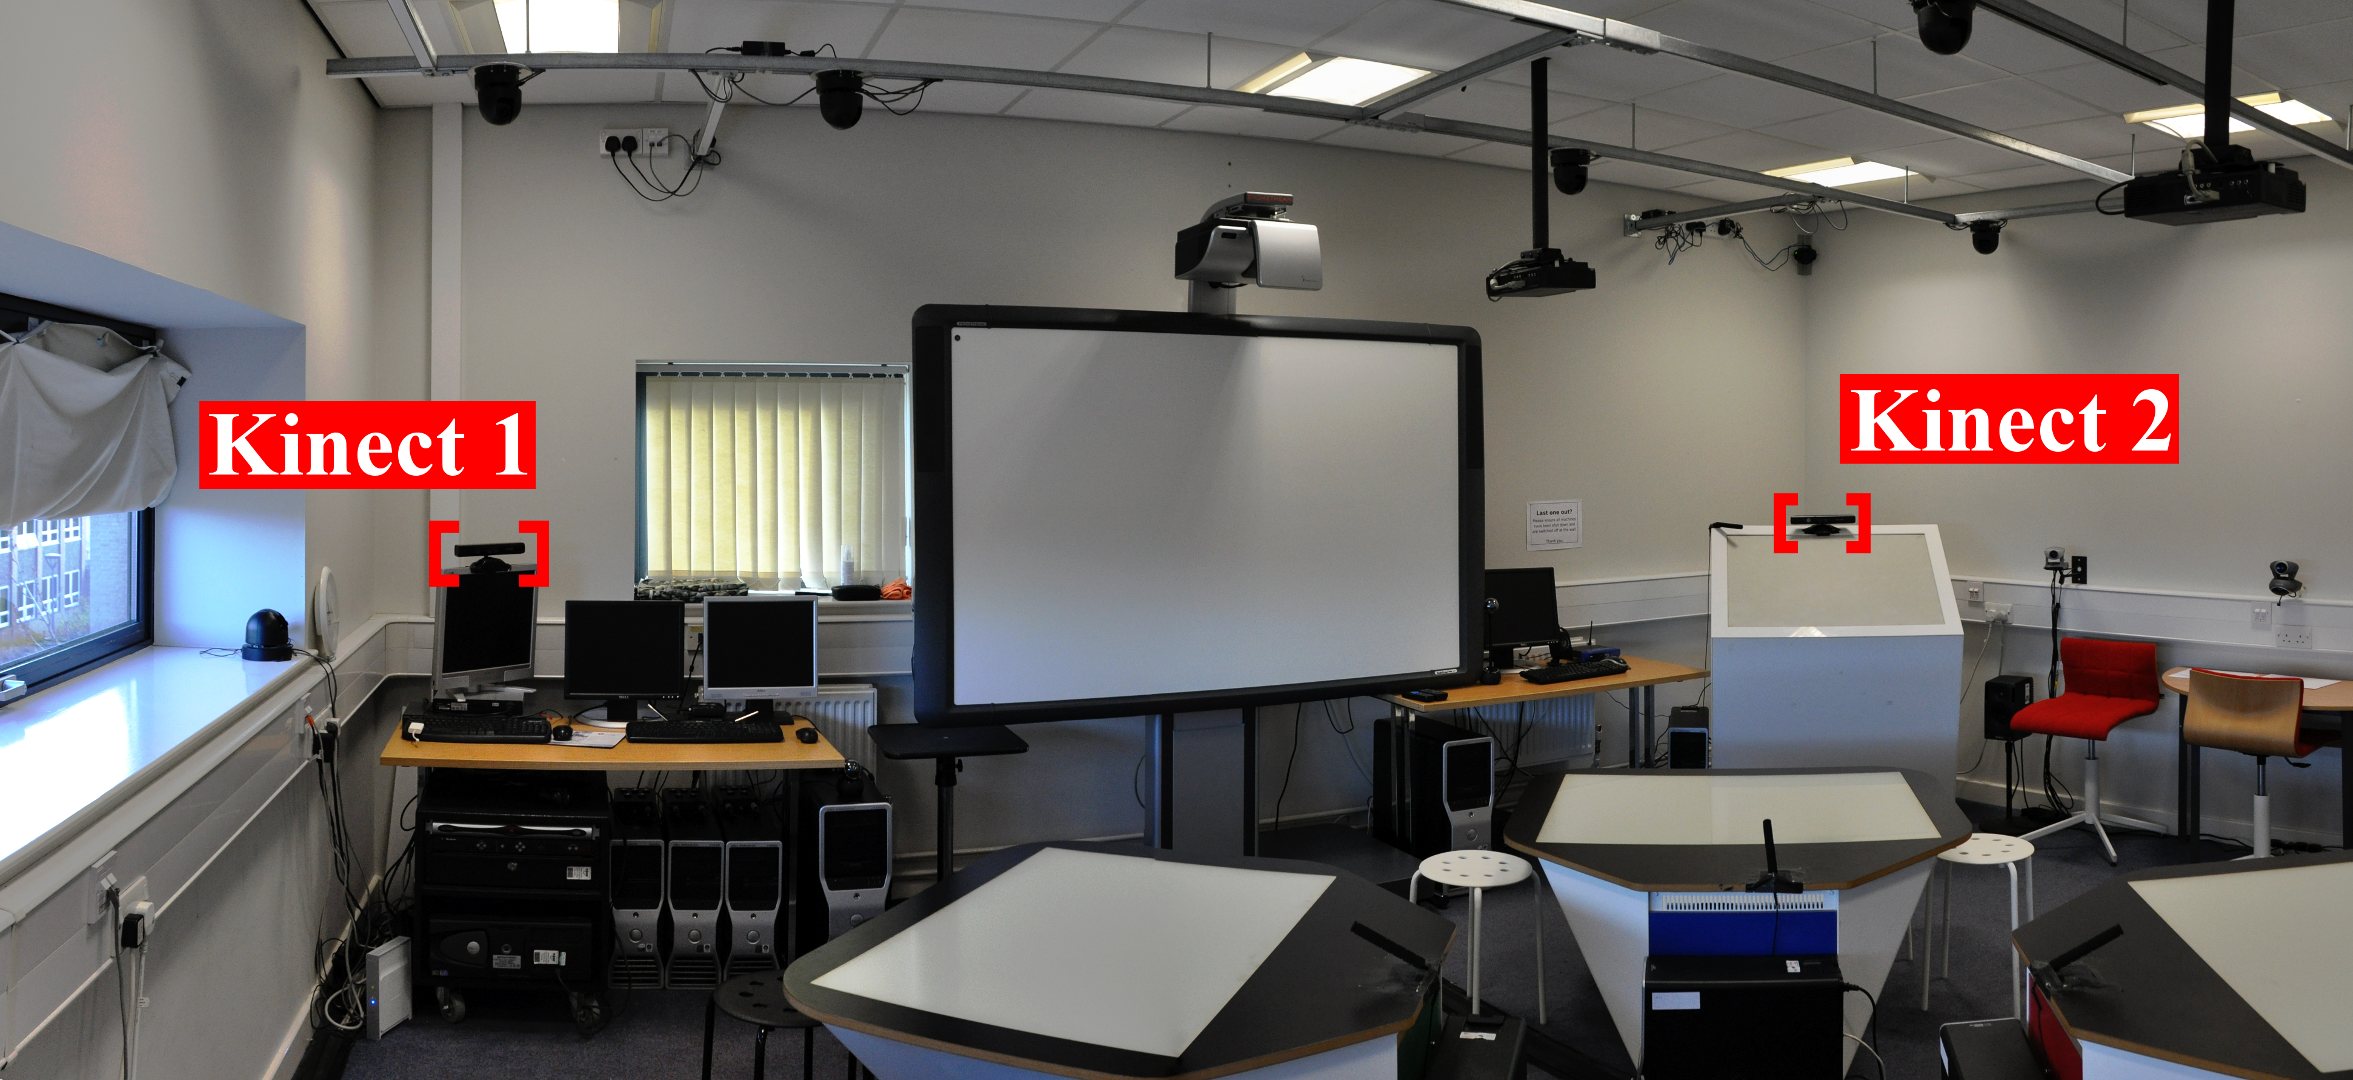
\includegraphics[width=0.45\textwidth]{figures/multiple_kinect_setup.png}
  \caption{The positioning of the two Kinects in the SynergyNet lab during the study.}
  \label{fig:kinectSetup}
\end{figure}

Figure~\ref{fig:kinectSetup} shows the positioning of the Kinect devices perpendicular to each other during the study.
This setup allowed for the entirety of the SynergyNet lab to be observed between the devices.

The study's primary hypothesis was that the use of the Kinects would allow for quicker and more frequent issuing of commands than the other two control technologies.
The secondary hypothesis was that the error rate of the Kinects would be similar to the error rates of the other two control technologies used in the study.

\subsubsection{Data Analysis}
\label{subsec:studyAnalysis}

The ordering of the tasks could have influenced the teacher's use of the system.
Gaining experience with the system commands during the earlier tasks may afford the teacher more confidence later in the study, theoretically reducing their error rate and improving their interaction times.
In addition to this, exposure to the system may have influenced the students.
Having gained familiarity with the student interfaces in earlier tasks the students may need less assistance from the teacher.
This may reduce the number of commands executed in the later tasks.
For these reasons the results focus on the times and errors per command rather than per task.

From the recordings the teacher's interactions with the various devices could be examined.
A time-line analysis tool, SynergyView~\cite{Kyaw2011}, was employed to annotate various interactions in the videos.
Each time the teacher attempted to issue a command with a control device an annotation was made.
The annotations note:
\begin{itemize}
\item The command the teacher wished to issue.
\item The control device used.
\item How long it took the teacher to issue the command (measured as the time from the teacher stating their intention for their next action to the time when the command was submitted).
\item Whether the command was issued successfully.
\item If unsuccessful whether the failure to issue the command was due to a technical fault or teacher-error.
\item If unsuccessful whether the command was a false positive (i.e. an unintentionally executed gesture acted upon by the system) or a false negative (i.e. a correctly executed gesture ignored by the system) where applicable.
\end{itemize}
With these annotations the average time taken to issue commands with each of the control devices can be calculated.
The frequency of each device's use and their error rates can also be identified through the video annotations.

\section{Results}
\label{sec:results}

The study was carried out without any major deviations from its design.
The teacher completed the training for the system several days before the study and stated that they felt confident enough to use the each of the control technologies without any additional aid or practice.

\subsection{Task 1: Board Only}
\label{subsec:resultsTask1}

For task 1 eleven commands were observed to be issued by the teacher in its 19 minute and 43 second duration.
Out of these eleven commands, one was issued incorrectly:

\begin{itemize}
\item This error was observed to occur when the teacher wished to freeze all tables.
When the freeze command was issued two tables were already frozen.
Because the command toggles the frozen state of an instance of SynergyNet, the two tables which were already frozen became unfrozen when the command was issued.
The teacher immediately recognised their mistake and issued a command from the board for specifically freezing the two, now unfrozen, interfaces.
This error was caused by the teacher's understanding of the system's functions and could have occurred with any of the controlling technologies.
\end{itemize}

\begin{figure}[h]
   \centering
   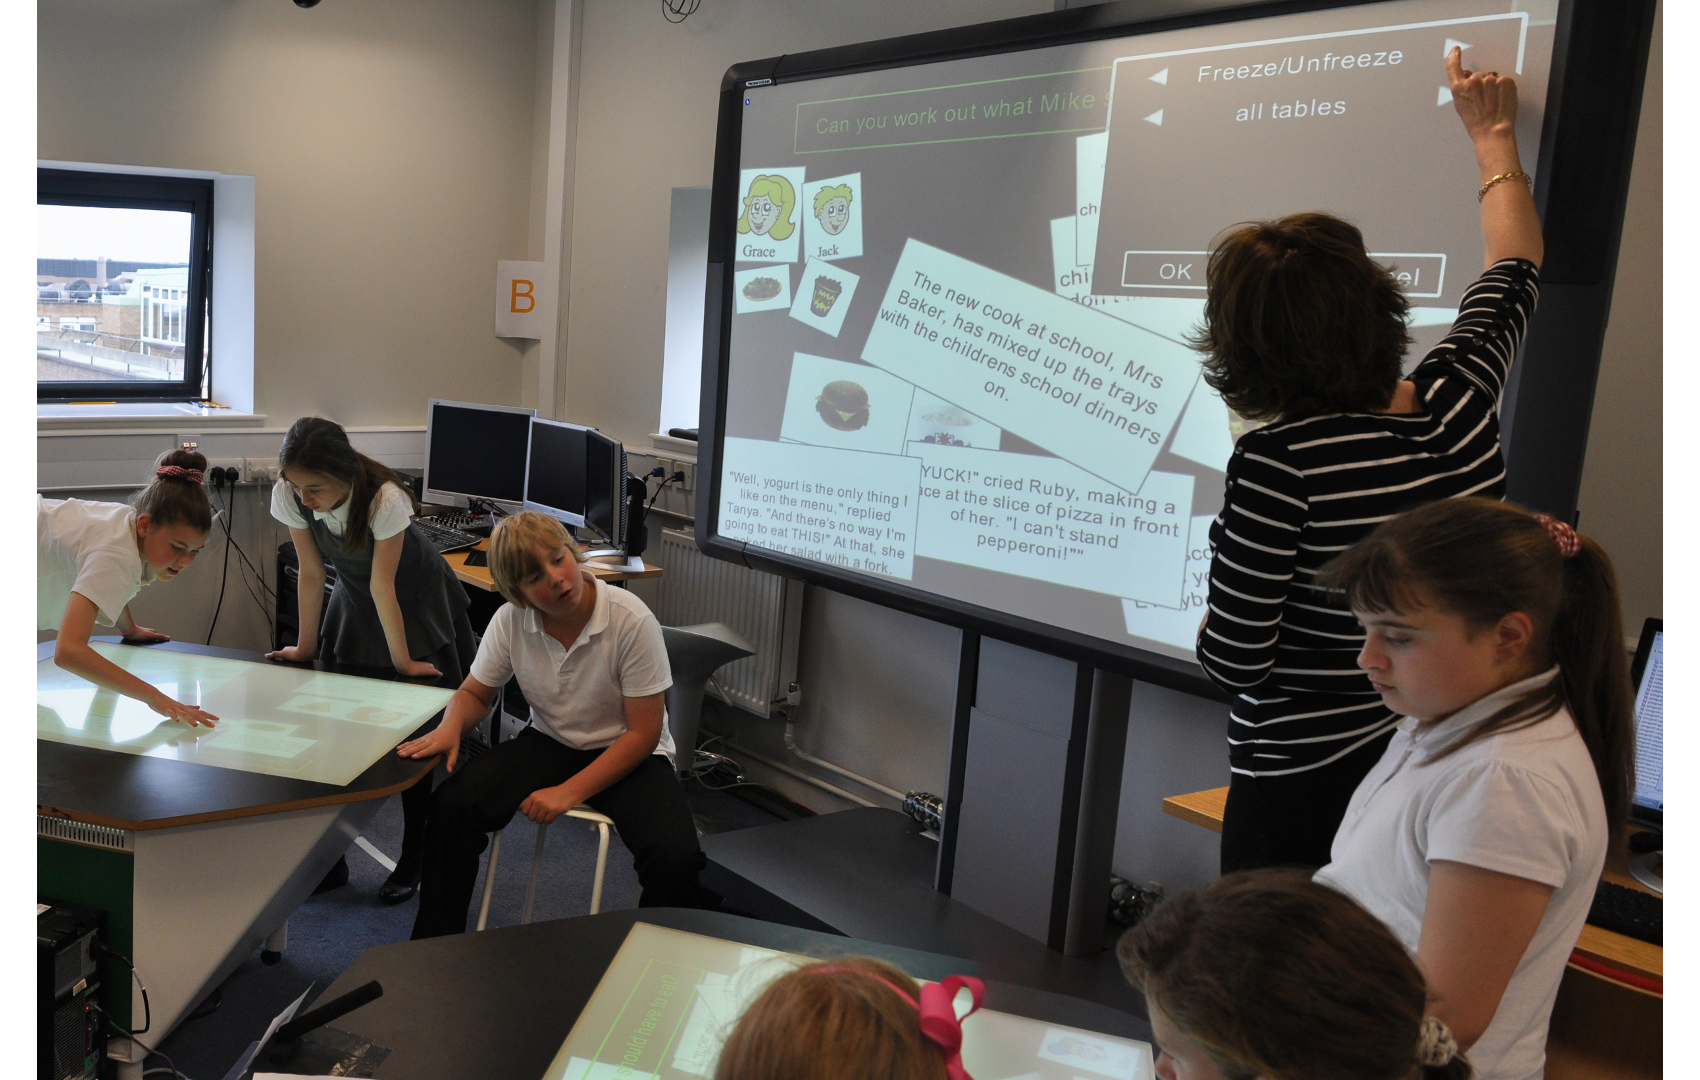
\includegraphics[width=0.45\textwidth]{figures/study_board.png}
   \caption{The board control in use during the study.}
   \label{fig:studyBoard}
\end{figure}

The average time taken to issue a successful command with the board was 9.82 seconds with a standard deviation of 5.97 seconds.
Six of the successful commands given were intended to affect all student interfaces and four were intended to affect a specific selection.

\subsection{Task 2: Tablet Only}
\label{subsec:resultsTask2}

During task 2, thirteen commands were observed to be issued by the teacher in its 17 minute and 59 second duration.
Of these thirteen commands, three were issued incorrectly.

\begin{itemize}
\item The first of these incorrectly issued commands occurred when the teacher wished to send content from one table to the board.
When this error was made obvious to the teacher by the wrong content appearing on the board they explained to their class that they'd accidentally selected more than one table.
The teacher confirmed this in the post-session interview.
It is apparent that the teacher had left other instances of SynergyNet selected when issuing an earlier command.
The controls accessed through the tablet don't reset the set of selected interfaces when a command is issued unlike the other two control technologies.
The teacher assumed that the tablet controls would behave like the board controls used in the pilot study and did not modify their usage accordingly.
This error can be attributed to the tablet's differing behaviour from the board and Kinect controls in regards to interface selection.

\item One of the erroneous commands observed during task 2 occurred when the teacher wished to issue a command to freeze all instances of SynergyNet on the student interfaces.
However, only a selection of the interfaces was frozen.
This was because the teacher did not update the selection criteria.
This is also due to the tablet controls' selection behaviour differing from the alternative technologies'.

\item The remaining error was caused by the teacher issuing a command intended to freeze all interface when several instances of SynergyNet were already frozen.
The outcome of this is that the already frozen SynergyNet instances become unfrozen.
This is a similar occurrence to the single erroneous command observed during task 1.
The teacher assumes that all the interfaces will be put into the same state of being frozen or unfrozen, not toggled from their current state.
This error could occur with any of the control technologies.
\end{itemize}

\begin{figure}[h]
   \centering
   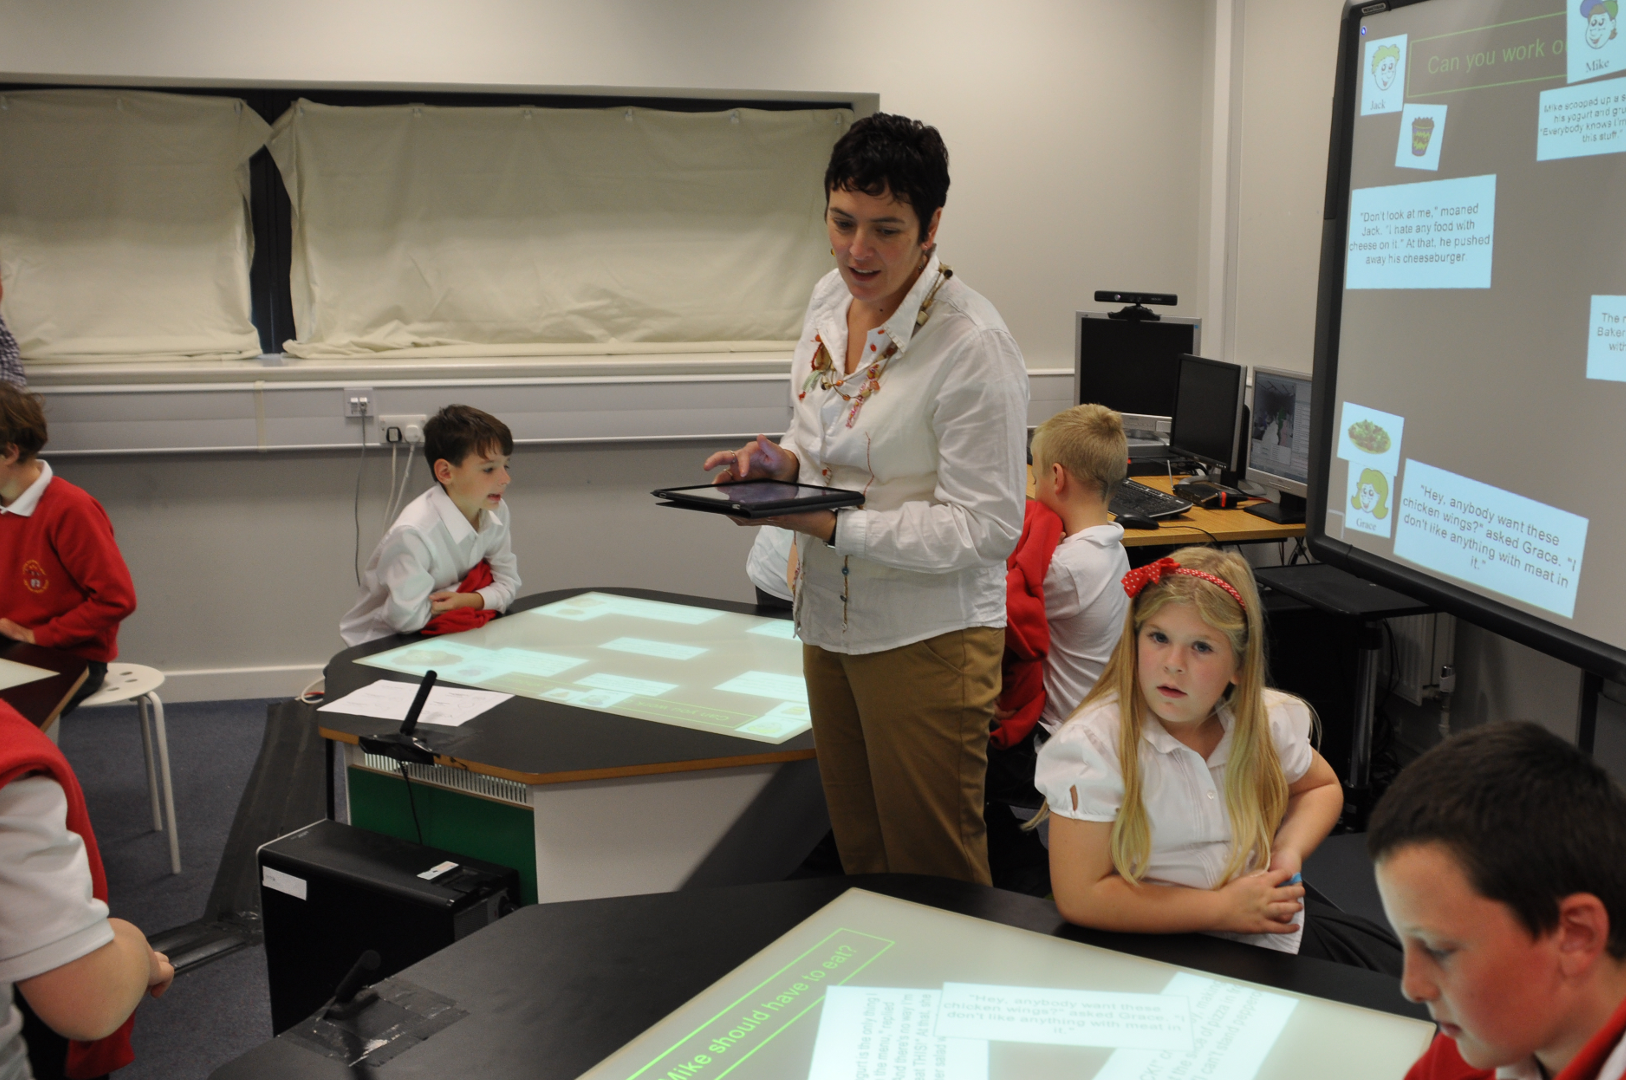
\includegraphics[width=0.45\textwidth]{figures/study_tablet.png}
   \caption{The web controls in use during the study, accessed through a tablet interface.}
   \label{fig:studyTablet}
\end{figure}

The average time taken to issue a successful command with the tablet was 9.17 seconds with a standard deviation of 13 seconds.
Eight of the successful commands given were intended to affect all student interfaces and two of the successful commands were intended to affect a specific selection.

\subsection{Task 3: Kinect Only}
\label{subsec:resultsTask3}

During task 3, twelve commands were observed to be issued by the teacher in its 18 minute duration.
Of the twelve commands issued during this task with the Kinects, eight were issued with errors.

\begin{itemize}
\item Three of these erroneous commands were observed to occur when the teacher wished to show content from a specific table.
Gaining attention and selecting the table both were problem free for these commands, the error occurred during the control gesture's execution.
To send content to the board the teacher needs to perform a push gesture.
This gesture was not identified by the Kinects and indicates a problem with the device's ability to track these occurrences of the gesture.

\item Two of the erroneous commands in task 3 occurred when the teacher intended to unfreeze all the tables.
The teacher successfully gained the device's attention both times but when they raised both hands for the control gesture the Kinects failed to track one of their arms.
The Kinects only see one arm in the air and interpret the command as the one used to dismiss its attention.
This appears to be a problem caused by the Kinects failing to correctly track the movement of a joint.

\item One of the commands which was issued with errors occurred when the teacher wished to transfer the content on the board to all the tables.
The teacher performed the pull gesture but did not perform the attention gaining gesture beforehand.
This meant that the Kinects ignored the teacher's command gesture.
This error occurred due to the teacher not following the control sequence.

\item Another of the erroneous commands was also observed to occur when the teacher intended to transfer content on the board to all of the student interfaces.
After successfully getting the Kinect's attention the teacher performs the pull gesture.
The Kinects did not see this movement correctly.
The teacher repeated the gesture several times but neither of the Kinects correctly tracked the movement of the hand before their attention timed out.
Instead, the Kinects would often assume that the moving arm was at rest by the teacher's side - a sign that the devices had lost track of the hand and arm joints.
This is another instance of a command made erroneous by the Kinects failing to track a joint accurately.

\item The final erroneous command occurred when the teacher intended to freeze all the student interfaces.
The teacher successfully gained the attention of the Kinect devices then stopped.
In the post-session interview the teacher revealed this was because they were trying to recall the control gesture because they had forgotten it.
The teacher did not resume the control sequence until after the Kinect nodes' attention timed out.
This error occurred due to the teacher not following the control sequence by pausing too long.
\end{itemize}

\begin{figure}[h]
   \centering
   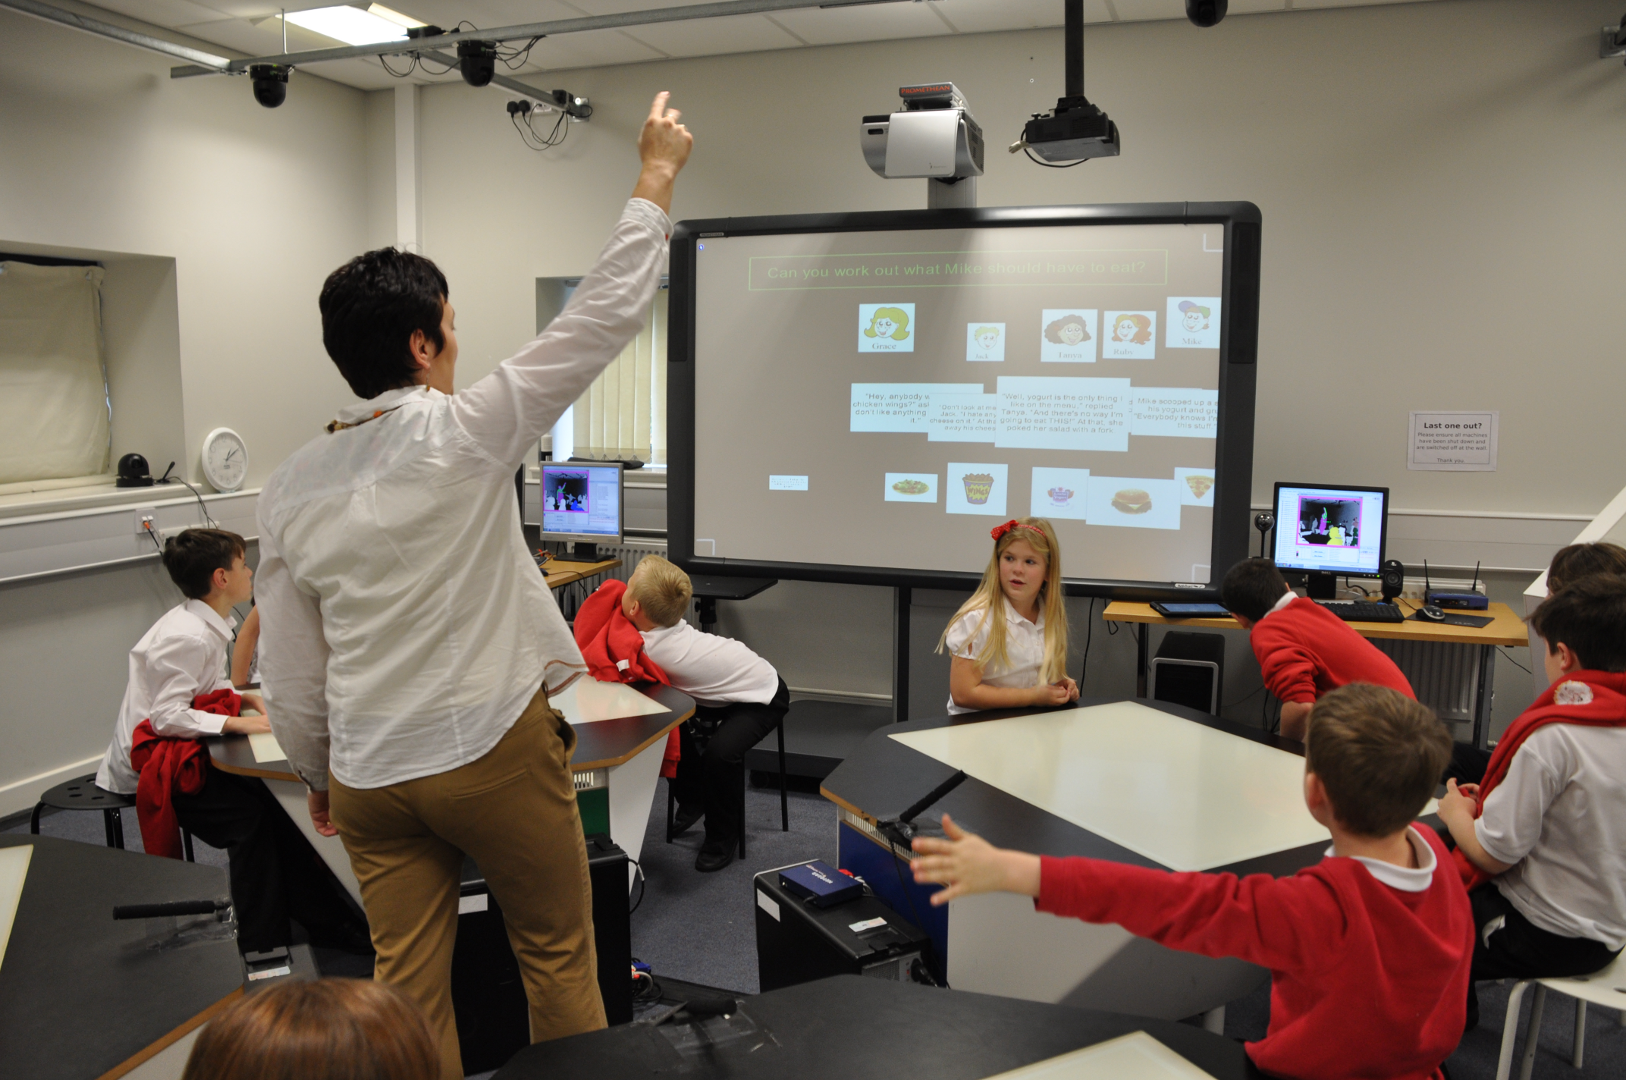
\includegraphics[width=0.45\textwidth]{figures/study_kinect.png}
   \caption{The Kinect control in use during the study.}
   \label{fig:studyKinect}
\end{figure}

The average time taken to issue a successful command with the Kinects was 2.44 seconds with a standard deviation of 0.54 seconds.
All four of the successful commands were intended to affect all the student interfaces.

\subsection{Task 4}
\label{subsec:resultsTask4}

For task 4, where the teacher had the option of using any of the three control devices, twenty three commands were observed to be issued by the teacher in its 19 minute and 28 second duration.
Nine of these commands were issued through the board control, none through the tablet and fourteen through the Kinects.
Out of these twenty three commands, five were issued incorrectly.
All five of these erroneous commands were issued using the Kinects.

\begin{itemize}
\item Two of the erroneous commands observed in task 4 occurred when the teacher attempted to display screenshots of all the student interfaces on the board.
The Kinects' attention was gained successfully but the devices both lost track of the teacher's right hand when the command gesture of holding two hands together was performed.
Like a number of erroneous commands observed during task 3, this failure to successfully identify a command gesture appears to result from the Kinects' joint tracking abilities.

\item One of the failures to successfully to issue a command occurred when the teacher intended to send content on the board to all tables.
After successfully obtaining the Kinects' attention the teacher performed the pulling gesture.
However, neither of Kinects was able to successfully interpret the movement of the hand as a command gesture.
The Kinects would show the arm moving to a resting position by the teacher's torso part way through the gesture, indicating that both of the devices had lost track of the hand and arm joints.
Again, this is an error caused by the Kinects' joint tracking.

\item Another of the erroneous commands observed during task 4 occurred when the teacher intended to freeze all the student interfaces.
The teacher successfully gained the devices' attention then performed the gesture of holding both hands up.
However, during the command gesture both the Kinects lost track of one of the teacher's hands, placing their left arm in a resting posting.
This had the consequence of only one arm being identified as in the air which was interpreted as the attention dismissing gesture.
This resulted in the teacher losing the Kinect's attention with no command being issued to the student interfaces.
This is yet another instance of the Kinect devices' tracking abilities causing errors.

\item The remaining erroneous command occurred when the teacher intended to send content from a specific table to the board.
After successfully gaining the attention of the Kinects the teacher performed the push command gesture.
Part way through the gesture the Kinects both interpreted the arm of the gesturing hand moving to a resting position.
This indicated that the Kinects had both lost track of the gesturing hand.
This is, again, an instance of the Kinects' tracking abilities causing a correctly performed command gesture to return erroneous results.
\end{itemize}

The average time taken to issue a successful command was 6.73 seconds with the board and 2.81 seconds with the Kinects.
The standard deviation was 3.29 seconds for the board and 1.51 seconds for the Kinects.
Seven of the successful commands given with the board were intended to affect all student interfaces and two of the successful board commands were intended to affect a specific selection.
For the Kinects, four of the successful commands given were intended to affect all student interfaces and five were intended to affect a specific selection.

\subsection{Results Summary}
\label{subsec:resultsSummary}

The usage of the three control technologies in the study is summarised in Table~\ref{table:results2}.

\begin{table}[h]
\centering
\begin{tabular}{!{\vrule width 1.5pt}c|c|c|c!{\vrule width 1.5pt}}
\noalign{\hrule height 1.5pt}
\multicolumn{1}{!{\vrule width 1.5pt}c!{\vrule width 1.5pt}}{\textbf{}}	
&\textbf{Number}
&\multicolumn{1}{!{\vrule width 1.5pt}c!{\vrule width 1.5pt}}{\textbf{Number}}	
&\textbf{Avg. time}\\
\multicolumn{1}{!{\vrule width 1.5pt}c!{\vrule width 1.5pt}}{\textbf{}}	
&\textbf{of}
&\multicolumn{1}{!{\vrule width 1.5pt}c!{\vrule width 1.5pt}}{\textbf{of}}	
&\textbf{to issue}\\
\multicolumn{1}{!{\vrule width 1.5pt}c!{\vrule width 1.5pt}}{\textbf{Device}}	
&\textbf{commands}
&\multicolumn{1}{!{\vrule width 1.5pt}c!{\vrule width 1.5pt}}{\textbf{errors}}	
&\textbf{commands}\\
\noalign{\hrule height 1.5pt}
Board 					&20 					&1				&8.28 seconds				\\
\cline{1-4}
Tablet 					&13					&3				&9.17 seconds				\\
\cline{1-4}
Kinect 					&26					&13			&2.63 seconds				\\
\noalign{\hrule height 1.5pt}
\end{tabular}
\caption{The usage of the control devices in the study.}
\label{table:results2}
\end{table}

\begin{figure}[h]
  \centering
  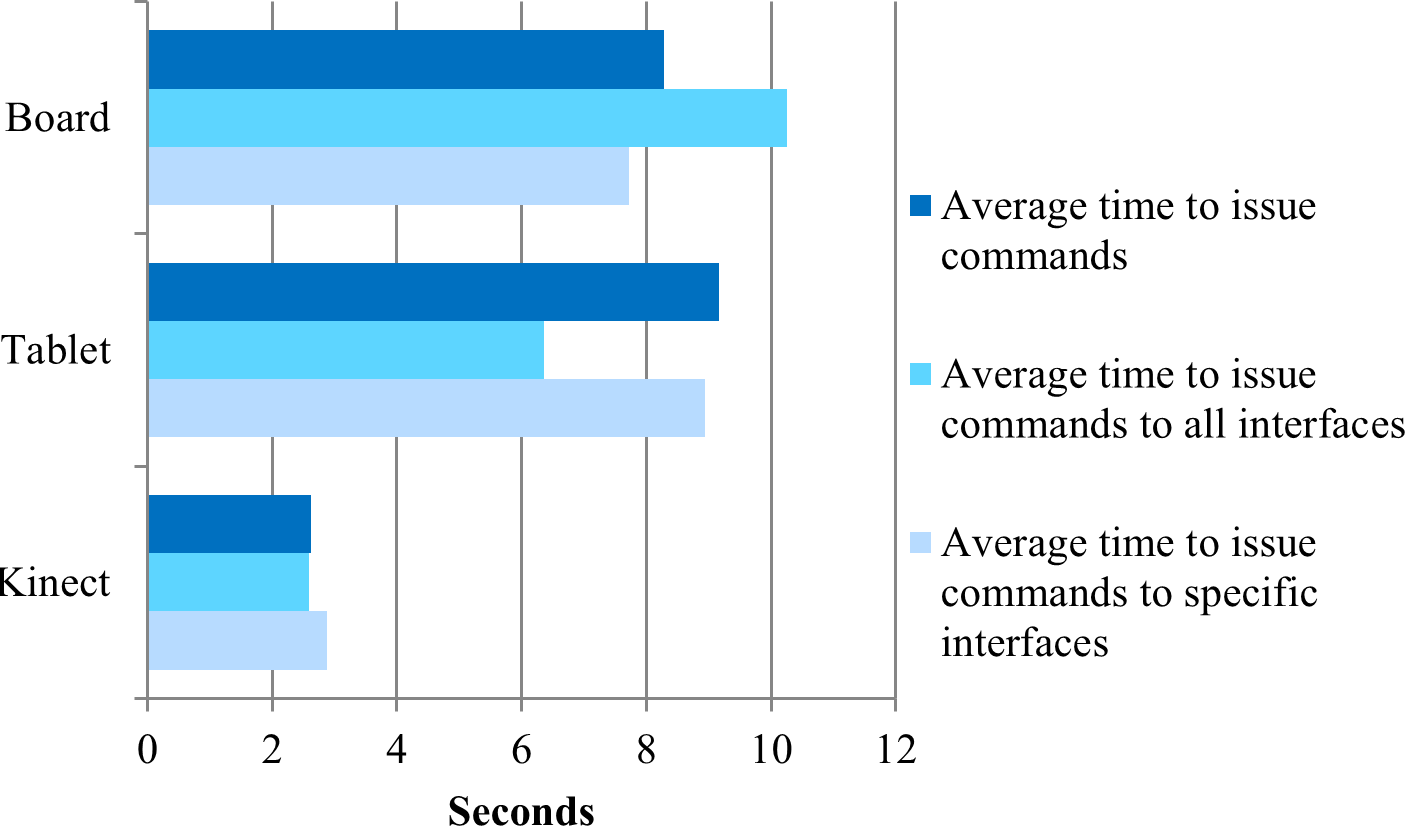
\includegraphics[width=0.45\textwidth]{figures/bar_chart_times.png}
  \caption{Comparison between the times taken to issue commands with each of the control technologies.}
  \label{fig:controlDevicesTimes}
\end{figure}

The results show that the Kinect was the much faster control technology for issuing commands, confirming the primary hypothesis of the study.
Figure~\ref{fig:controlDevicesTimes} highlights how this was consistent across those intended for specific or all interfaces too.
However, the Kinect had a much higher error-rate than the other two control technologies disproving the study's secondary hypothesis.

\subsection{Reviewing Improvements}
\label{subsec:reviewingImprovements}

Despite the improvements intended to improve device accuracy and range, the majority of errors observed in the study originated from the Kinect devices themselves.
Eleven of the thirteen unsuccessful commands executed with the Kinect controls were made erroneous due to the Kinect devices losing track of a joint.

The implementation of a more cohesive gesture set appears to have been a successful improvement to the system.
The results of the study show that the teacher never confused any of the gestures.
In addition to this the teacher rarely had any problems recalling a specific command, only once pausing for a significant amount of time to recall one.

Enabling pause tolerance in the control sequence appears to have improved the system.
Only one erroneous command resulted from a teacher's movements between stages of the control sequence.

Implementing automatic calibration appears to have had its intended effect of simplifying the control sequence to aid intuitiveness and mental load requirements.
The teacher never needed to perform the calibration pose, saving time and reducing the amount of teacher input required by the system.
This simplification of the control sequence may have resulted in the teacher only once performing the steps needed to issue a command incorrectly.

The implemented improvement of interface selection had its intended effect of enabling a teacher to select which tables a command would affect.
There were no errors observed during the table selection phase of all the commands issued throughout the study.

\section{Conclusions}
\label{sec:conclusions}

\begin{figure}[h]
   \centering
   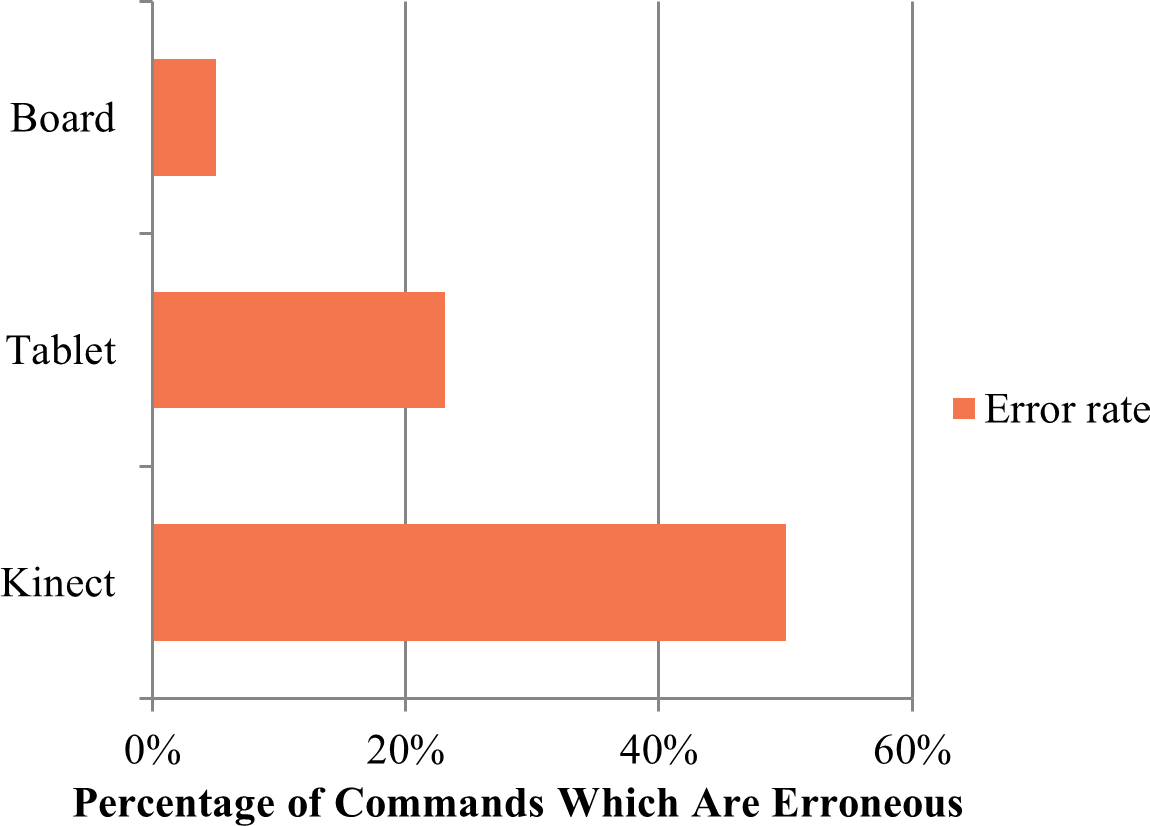
\includegraphics[width=0.45\textwidth]{figures/bar_chart_errors.png}
   \caption{Comparison between the error rates of each of the control technologies.}
   \label{fig:controlDevicesErrors}
 \end{figure}

In the pilot study the Kinect controls had an overall error rate of 86\%
As Figure~\ref{fig:controlDevicesErrors} shows, the error rate for the Kinect controls in the study was 50\%.
This indicates that the improvements outlined in Section~\ref{sec:resolvingIssuesObserved} which were implemented into the study, as outlined in Section\ref{subsec:studyImplementation}, had a beneficial impact of the use of the gesture control sequence.

The 50\% error rate indicates that there are still issues with the implementation which could be improved upon in the future.

The issue of the Kinect devices losing track of user's limbs and joints remains a significant source of errors despite the improvements made after the pilot study.
Of the thirteen erroneous commands issued with the Kinect observed to occur in the study, the failure of eleven of these commands was attributed to the devices losing track of users' joints.
All of these occurrences observed to occur when the teacher's body was entirely within the device's range.
This indicates that limited interaction space was not the cause of the tracking problems.
It appears the Kinect has issues which tracking the movement of the teacher's arms during specific gestures.
It is likely this may be caused by the speed at which the gesture is executed~\cite{Winkler2012}.
The majority of the gestures affected appeared to be those which required the movement of a hand.
This indicates that the Kinect may have issues with tracking movement of limbs precisely enough for some of the gestures used in the control sequence, such as push and pull gestures.

Another cause for the inaccurate tracking could be occlusion~\cite{Meng2012}.
Movement by the teacher during a gesture may momentarily obscure the tracked joints from the Kinect's view.
While a joint is momentarily obscured from view the Kinect may assume it has moved to a resting position.
This was observed to occur several times during the study.
This movement of an arm mid gesture to a resting position changes the gesture's perceived movement in such a way that SynergyNet will not recognise the gesture.
Though two Kinects observe each gesture, a brief occlusion of the tracked joints on both systems during the teacher's movement (not necessarily at the same time) will break their recognition of the gesture.
Future improvements could involve an algorithm to smooth movement and ignore frames where limbs and joints are observed to be somewhere unexpected.
The challenge of this proposed improvement will be implement it in such a way that it does not reduce the responsiveness of the system by too much.

The results of the study demonstrated that the Kinect was the quickest control technology for issuing commands from which shows it has potential as an orchestration tool in the classroom.
In addition to this the teacher who participated in the study expressed a preference for the Kinect in the post session interview due to the speed and freedom it offered.

85\% of the errors which occurred in the study were attributed to the Kinect devices' losing track of user limbs.
If the issue of the Kinect losing track of joints was resolved, the error rate would be significantly reduced.
If the errors relating to accuracy had not occurred during the study the error rate would have been 8\%.
Because the remaining errors were deemed to be minor because of their minimal negative consequences the system could be considered fit for purpose.
It is apparent that a method of improving the accuracy of the system's joint tracking is required.

The other improvements implemented into SynergyNet after the pilot study appear to have been successful.
Errors where the accuracy of the Kinects was not concerned which were observed during the pilot study were not observed to occur in the main study.
These improvements could be considered in other open-air gesture systems which could potentially suffer from the same issues.

The accuracy of the Kinect devices resulted in the system being made unfit for purpose.
If this issue was resolved the system would be a viable classroom technology control system.
The speed of commands issued using gestures and lack of errors outside of those caused by the accuracy of the technology used compared to the more traditional orchestration technologies used show huge benefits in using a light-coding device like the Kinect.
This indicates that gestures can be a viable method for controlling technology in the classroom if the appropriate improvements are made.

\begin{ack}

This work was partially funded under the UK's EPSRC/ERSC Teaching and Learning Research Programme (TLRP) {\emph{SynergyNet}} project (RES-139-25-0400).
The authors would also like to thank the members of the Durham University Technology Enhanced Learning Special Interest Group for supporting the redrafting of this manuscript, specifically Andrew Joyce-Gibbons.
The source code for the software implemented in the studies discussed in this manuscript is freely available here: \url{https://github.com/synergynet/synergynet3.1}.

\end{ack}

\makeatletter
\def\@biblabel#1{}
\makeatother

% Bibliography
\bibliographystyle{apa}
\bibliography{kinectpaper}

\end{document}
